\g
\chapter{Θεωρητικό μέρος - Στερεοσκοπική όραση}
\label{Chapter2}

\section{Σχηματισμός εικόνας μέσω της προοπτικής προβολής}

Έστω χώρος σημείων $A$. Εάν σε αυτόν προσδιορίσουμε μια γραμμικώς ανεξάρτητη βάση $ V $ και μια αρχή $ o \in A $, τότε έχει οριστεί ένα σύστημα συντεταγμένων του χώρου σημείων $A = (o,V) $. Υπάρχει ισομορφισμός μεταξύ του $A = (o,V) $ και του συνόλου $\mathbb{R}^n$. Στην περίπτωση του τρισδιάστατου φυσικού κόσμου ο ισομορφισμός ικανοποιείται με το σύνολο $\mathbb{R}^3$. Πλέον, κάθε σημείο $ p = o \bigoplus v $ του χώρου $Α$, δηλαδή του τρισδιάστατου κόσμου, μπορεί να περιγραφεί μονοσήμαντα μέσω 3 συντεταγμένων $ \mathbf{P} = (X,Y,Z)$ που είναι οι συντεταγμένες του $v$ ως προς την προαναφερθείσα συγκεκριμένη βάση. 
 
Η εικόνα αποτελεί την θέαση του τρισδιάστατου κόσμου σε δύο διαστάσεις. Μαθηματικά είναι μια συνάρτηση $$ f : \mathbb{R}^3 \rightarrow \mathbb{R}^2 $$ η οποία μετασχηματίζει τις τρισδιάστατες συντεταγμένες του τυχαίου σημείου $\mathbf{P} = (X,Y,Z)$ στις $ \mathbf{p} = (x,y)$. Η πιο γνωστή μέθοδος προβολής είναι η προοπτική και με αυτήν θα ασχοληθούμε στην παρούσα εργασία.

Η προοπτική προβολή συνίσταται στην "1-1" αντιστοίχηση \e(mapping)\g των σημείων του χώρου στο πέτασμα της κάμερας αν μιλάμε για ένα τεχνητό οπτικό μέσο ή στον χιτώνα του ματιού αν εξετάζουμε το οπτικό μέσο του ανθρώπου. Η αντιστοίχηση υλοποιείται μέσω του μοντέλου "κάμερας μικρής οπής" \e (pinhole model). \g 

Η $f_{pr}$ περιγράφεται ποιοτικά από την παρακάτω μη γραμμική συνάρτηση:\footnote{Πληρέστερη μοντελοποίηση της προοπτικής προβολής δίνεται στο παράρτημα \ref{appendix:extensive_projection}}

\begin{equation}
	\mathbf{p} = f_{pr}(\mathbf{P}) : (x,y) = \left(f\frac{X}{Z}, f\frac{Y}{Z}\right)
\end{equation} 

η οποία εκφράζεται και σε μορφή πινάκα με την χρήση ομογενών συντεταγμένων:

\begin{equation}
Z\begin{bmatrix}x \\ y \\ 1\end{bmatrix} = 
\begin{bmatrix}
f & 0 & 0 & 0\\
0 & f & 0 & 0\\
0 & 0 & 1 & 0 
\end{bmatrix} 
\begin{bmatrix}
X \\ Y \\ Z \\ 1
\end{bmatrix}
\end{equation}

Η προοπτική προβολή είναι \emph{μη} αντιστρεπτή πράξη: 

$$ \nexists f_{pr}^{-1} : \lbrace\mathbb{R}^2 \rightarrow \mathbb{R}^3\rbrace : \mathbf{P} = f_{pr}^{-1}(\mathbf{p}) \Leftrightarrow (X,Y,Z) = f_{pr}^{-1}(x,y) $$

Πρακτικά αυτό σημαίνει ότι για κάθε σημείο $\mathbf{p}$ του πετάσματος της κάμερας είναι αδύνατος ο προσδιορισμός του σημείου $\mathbf{P}$ του τρισδιάστατου χώρου από το οποίο προήλθε. Γνωρίζουμε ότι οι υποψήφιες θέσεις του σημείου $\mathbf{P}$ κινούνται στην ευθεία που ενώνει το οπτικό κέντρο $O$ της κάμερας με το σημείο $\mathbf{p}$. Διανυσματικά η ευθεία αυτή περιγράφεται από την έκφραση:\footnote{Πληρέστερη έκφραση της ευθείας δίνεται στο παράρτημα \ref{appendix:extensive_projection_line}}

\begin{equation} \label{eq:simple_line}
\mathbf{l} = (X,Y,Z) = t\cdot \left (\dfrac{x}{f}, \dfrac{y}{f}, 1\right),  t \in [f,+\infty)
\end{equation}

Ερμηνεύοντας το αποτέλεσμα αντίστροφα, οποιοδήποτε σημείο $\mathbf{P}$ που ανήκει στην ευθεία $\mathbf{l}$ θα προβληθεί στο ίδιο ακριβώς σημείο $ \mathbf{p} $ του πετάσματος. 

Όπως παραστατικά αποτυπώνεται στην εικόνα \ref{fig:illusion} και μαθηματικά στην εξίσωση \ref{eq:simple_line}, δεν αρκεί μια εικόνα για την ακριβή ανάκτηση της αρχικής τρισδιάστατης πληροφορίας.


\begin{figure}
	\centering
	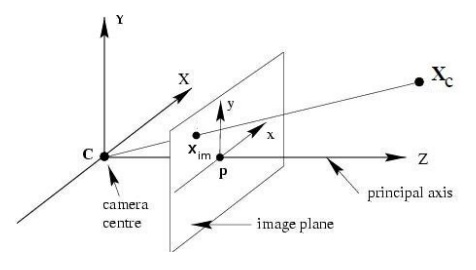
\includegraphics[scale=0.7]{perspective_projection}
	\caption{Γεωμετρική απεικόνιση της προοπτικής προβολής σημείου.}
	\label{fig:persp_proj}
\end{figure}

\begin{figure}
	\centering
	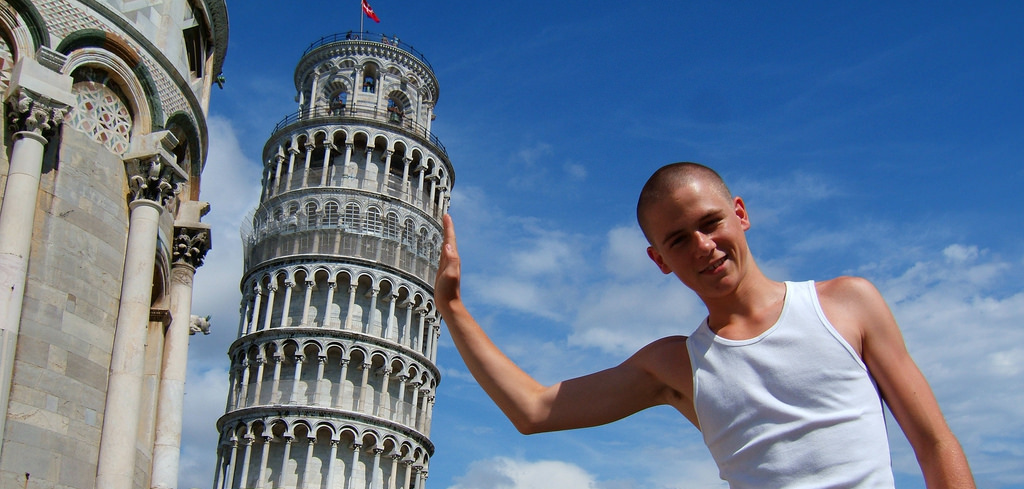
\includegraphics[scale=0.4]{illusion}
	\caption{Η ανάκτηση του βάθους είναι μια δύσκολη υπόθεση}
	\label{fig:illusion}
\end{figure}


%%%%%%%%%%%%%%%%%%%%%%%%%%%%%%%%%%%%%%%%%%%%%%%%%%%%%%%%%%%%%%%%%%%%%%%%%%%%%%%%%%%%%%%%%%%%%%%
\section{Γεωμετρία πολλαπλών προβολών}

Στην γεωμετρία πολλαπλών προβολών διαθέτουμε $n\geq2$ λήψεις της ίδιας τρισδιάστατης σκηνής. Θα μας απασχολήσει η περίπτωση των $n=2$ λήψεων.

\subsection{Προσδιορισμός τρισδιάστατης θέσης σημείου από δύο λήψεις}

Υποθέτουμε ότι:

\begin{enumerate}
	\item Ως σύστημα αναφοράς έχουμε ορίσει το σύστημα συντεταγμένων της μία εκ των δύο λήψεων. Την λήψη αυτή την ονομάζουμε λήψη αναφοράς και στην παρούσα εργασία επιλέγουμε να είναι η αριστερή.
	\item Γνωρίζουμε την ακριβή θέση και τον προσανατολισμό της έτερης (δεξιάς) λήψης στο χώρο. Συγκεκριμένα για τον πλήρη προσδιορισμό μιας λήψης ως προς μια άλλη χρειάζονται ένας πίνακα περιστροφής $R \in \mathbb{R}^{3\times 3} : \parallel R\parallel = 1$ και ένας πίνακας μετατόπισης $T \in  \mathbb{R}^3$. Αυτοί οι δύο πίνακες μαζί συνθέτουν έναν μετασχηματισμό \e affine, \g που τον συμβολίζουμε ως $g = (R,T)$. Εάν γνωρίζουμε τις συντεταγμένες ενός τυχαίου σημείου $P$ ως προς ένα ορισμένο σύστημα συντεταγμένων (στην περίπτωσή μας της αριστερής κάμερας), μπορούμε μέσω του μετασχηματισμού \e affine \g $g$ να βρούμε τις συντεταγμένες του $P$ ως το σύστημα συντεταγμένων της δεξιάς κάμερας. 
	\item Γνωρίζουμε τις ακριβείς θέσεις $ \mathbf{p_l}, \mathbf{p_r} \in \mathbb{R}^2$ στις οποίες έχει προβληθεί το \emph{ίδιο} σημείο του τρισδιάστατου χώρου $\mathbf{P}$.
\end{enumerate}

Με χρήση της σχέσης \ref{eq:simple_line}, προκύπτουν οι τρισδιάστατες \emph{ομοεπίπεδες} ευθείες $l_1$ και $l_2$ που αναλογούν στα σημεία $\mathbf{p_l}$ και $\mathbf{p_r}$. Το σημείο τομής των δύο ευθειών είναι η αρχική θέση $\mathbf{P}$ των σημείων $\mathbf{p_l}, \mathbf{p_r}$. Η διαδικασία αυτή, που φαίνεται στην εικόνα \ref{fig:triangulation}, ονομάζεται τριγωνοποίηση \e (triangulation). \g

\begin{figure}
	\centering
	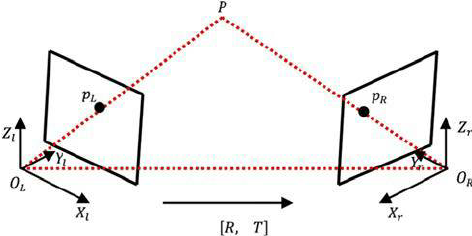
\includegraphics[scale=0.6]{triangulation}
	\caption{Τριγωνοποίηση}
	\label{fig:triangulation}
\end{figure}

\subsection{Το πρόβλημα της αντιστοίχησης}

Η μέθοδος της τριγωνοποίησης προϋποθέτει την γνώση των σημείων $\mathbf{p_l}$ και $\mathbf{p_r}$\footnote{στο εξής θα αναφέρονται ως "αντίστοιχα σημεία"}. Επομένως για την ανάκτηση της τρισδιάστατης θέσης ενός τυχαίου σημείου $\mathbf{p_l}$ απαιτείται η ανεύρεση του αντίστοιχου σημείου του $\mathbf{p_r}$ στην έτερη λήψη. Αυτή η αναζήτηση, που ονομάζεται "πρόβλημα αντιστοίχησης" \e (correspodence problem), \g είναι το κυρίαρχο πρόβλημα προς επίλυση σε κάθε εφαρμογή ανακατασκευής τρισδιάστατης πληροφορίας. 

Η αναζήτηση του "αντίστοιχου σημείου" δεν γίνεται κατά τυχαίο τρόπο στο σύνολο της έτερης λήψης. Αντίθετα η γεωμετρία των δύο προβολών περιορίζει την αναζήτησή του κατά μήκος μιας συγκεκριμένης ευθείας που βρίσκεται στο πέτασμα της έτερης λήψης. Η ευθεία αυτή ονομάζεται "επιπολική ευθεία". 

Αρχικά ορίζεται ο πίνακας \e essential matrix \g ως:

$$ E = [T]R \in \mathbb{R}^{3\times3}$$

Ως $[T]$ συμβολίζουμε τον $3\times 3$ πίνακα εξωτερικού γινομένου του διανύσματος $T$. Ο \e essential matrix \g υπολογίζεται άμεσα εφόσον γνωρίζουμε τον \e affine \g μετασχηματισμό $g = (R,T)$ και συμπυκνώνει την γεωμετρική συσχέτιση των σημείων $\mathbf{p_l}$ και $\mathbf{p_r}$ καθώς ικανοποιεί την σχέση:\footnote{Η απόδειξη της σχέσης \ref{eq:epipolar_constraint} παρατίθεται αναλυτικά στο παράρτημα \ref{appendix:epipolar_constraint_proof}}

\begin{equation} \label{eq:epipolar_constraint}
	\mathbf{p_r}^{T} E \mathbf{p_l} = 0
\end{equation}

Η σχέση \ref{eq:epipolar_constraint} ονομάζεται στερεοσκοπικός περιορισμός και από αυτήν προκύπτουν οι "επιπολικές ευθείες" κατά μήκος των οποίων βρίσκονται οι υποψήφιες θέσεις του "αντίστοιχου σημείου". Συγκεκριμένα εάν συμβολίσουμε με έναν πίνακα-γραμμή $l=[a \: b \: c]$ μια τυχαία ευθεία του επιπέδου $\mathbb{R}^2$\footnote{Έτσι ώστε το εσωτερικό γινόμενο του διανύσματος ευθείας $\mathbf{l}$ και ενός σημείου $\mathbf{p}$ να κάνει μηδέν μόνο όταν το σημείο ανήκει στην ευθεία} τότε ισχύει: 

\begin{itemize}

	\item το "αντίστοιχο σημείο" του $\mathbf{p_r}$ θα βρίσκεται πάνω στην επιπολική ευθεία $l_l = \mathbf{p_r}^{T} Ε$. Η ευθεία $l_l$ ορίζεται ως προς το σύστημα αναφοράς της λήψης 1 και βρίσκεται πάνω στο επίπεδο του πετάσματος της κάμερας 1, δηλαδή το επίπεδο $z = f$.
	\item το "αντίστοιχο σημείο" του $\mathbf{p_l}$ θα βρίσκεται πάνω στην επιπολική ευθεία $l_r = \mathbf{p_l} Ε$. Η ευθεία $l_r$ ορίζεται ως προς το σύστημα αναφοράς της λήψης 2 και βρίσκεται πάνω στο επίπεδο του πετάσματος της κάμερας 2, δηλαδή το επίπεδο $z = f$.
\end{itemize}

\begin{figure}
	\centering
	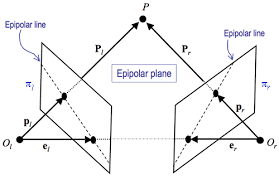
\includegraphics[scale=1]{epipolar_line}
	\caption{Επιπολικό επίπεδο και επιπολική ευθεία}
	\label{fig:epipolar_line}
\end{figure}


\subsection{Αντιστοίχηση στη στερεοσκοπική όραση}

\begin{figure}
	\centering
	\begin{subfigure}{0.48\textwidth}
		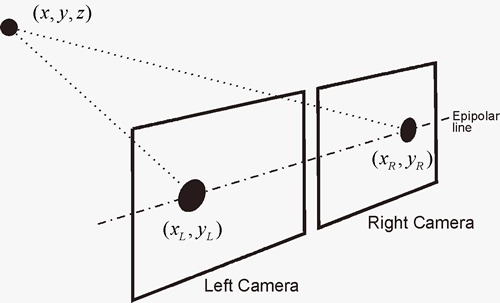
\includegraphics[width=\textwidth]{stereo_geometry}
		\caption{Στερεοσκοπική γεωμετρία}
		\label{fig:stereo_geometry}
	\end{subfigure}
	\begin{subfigure}{0.48\textwidth}
		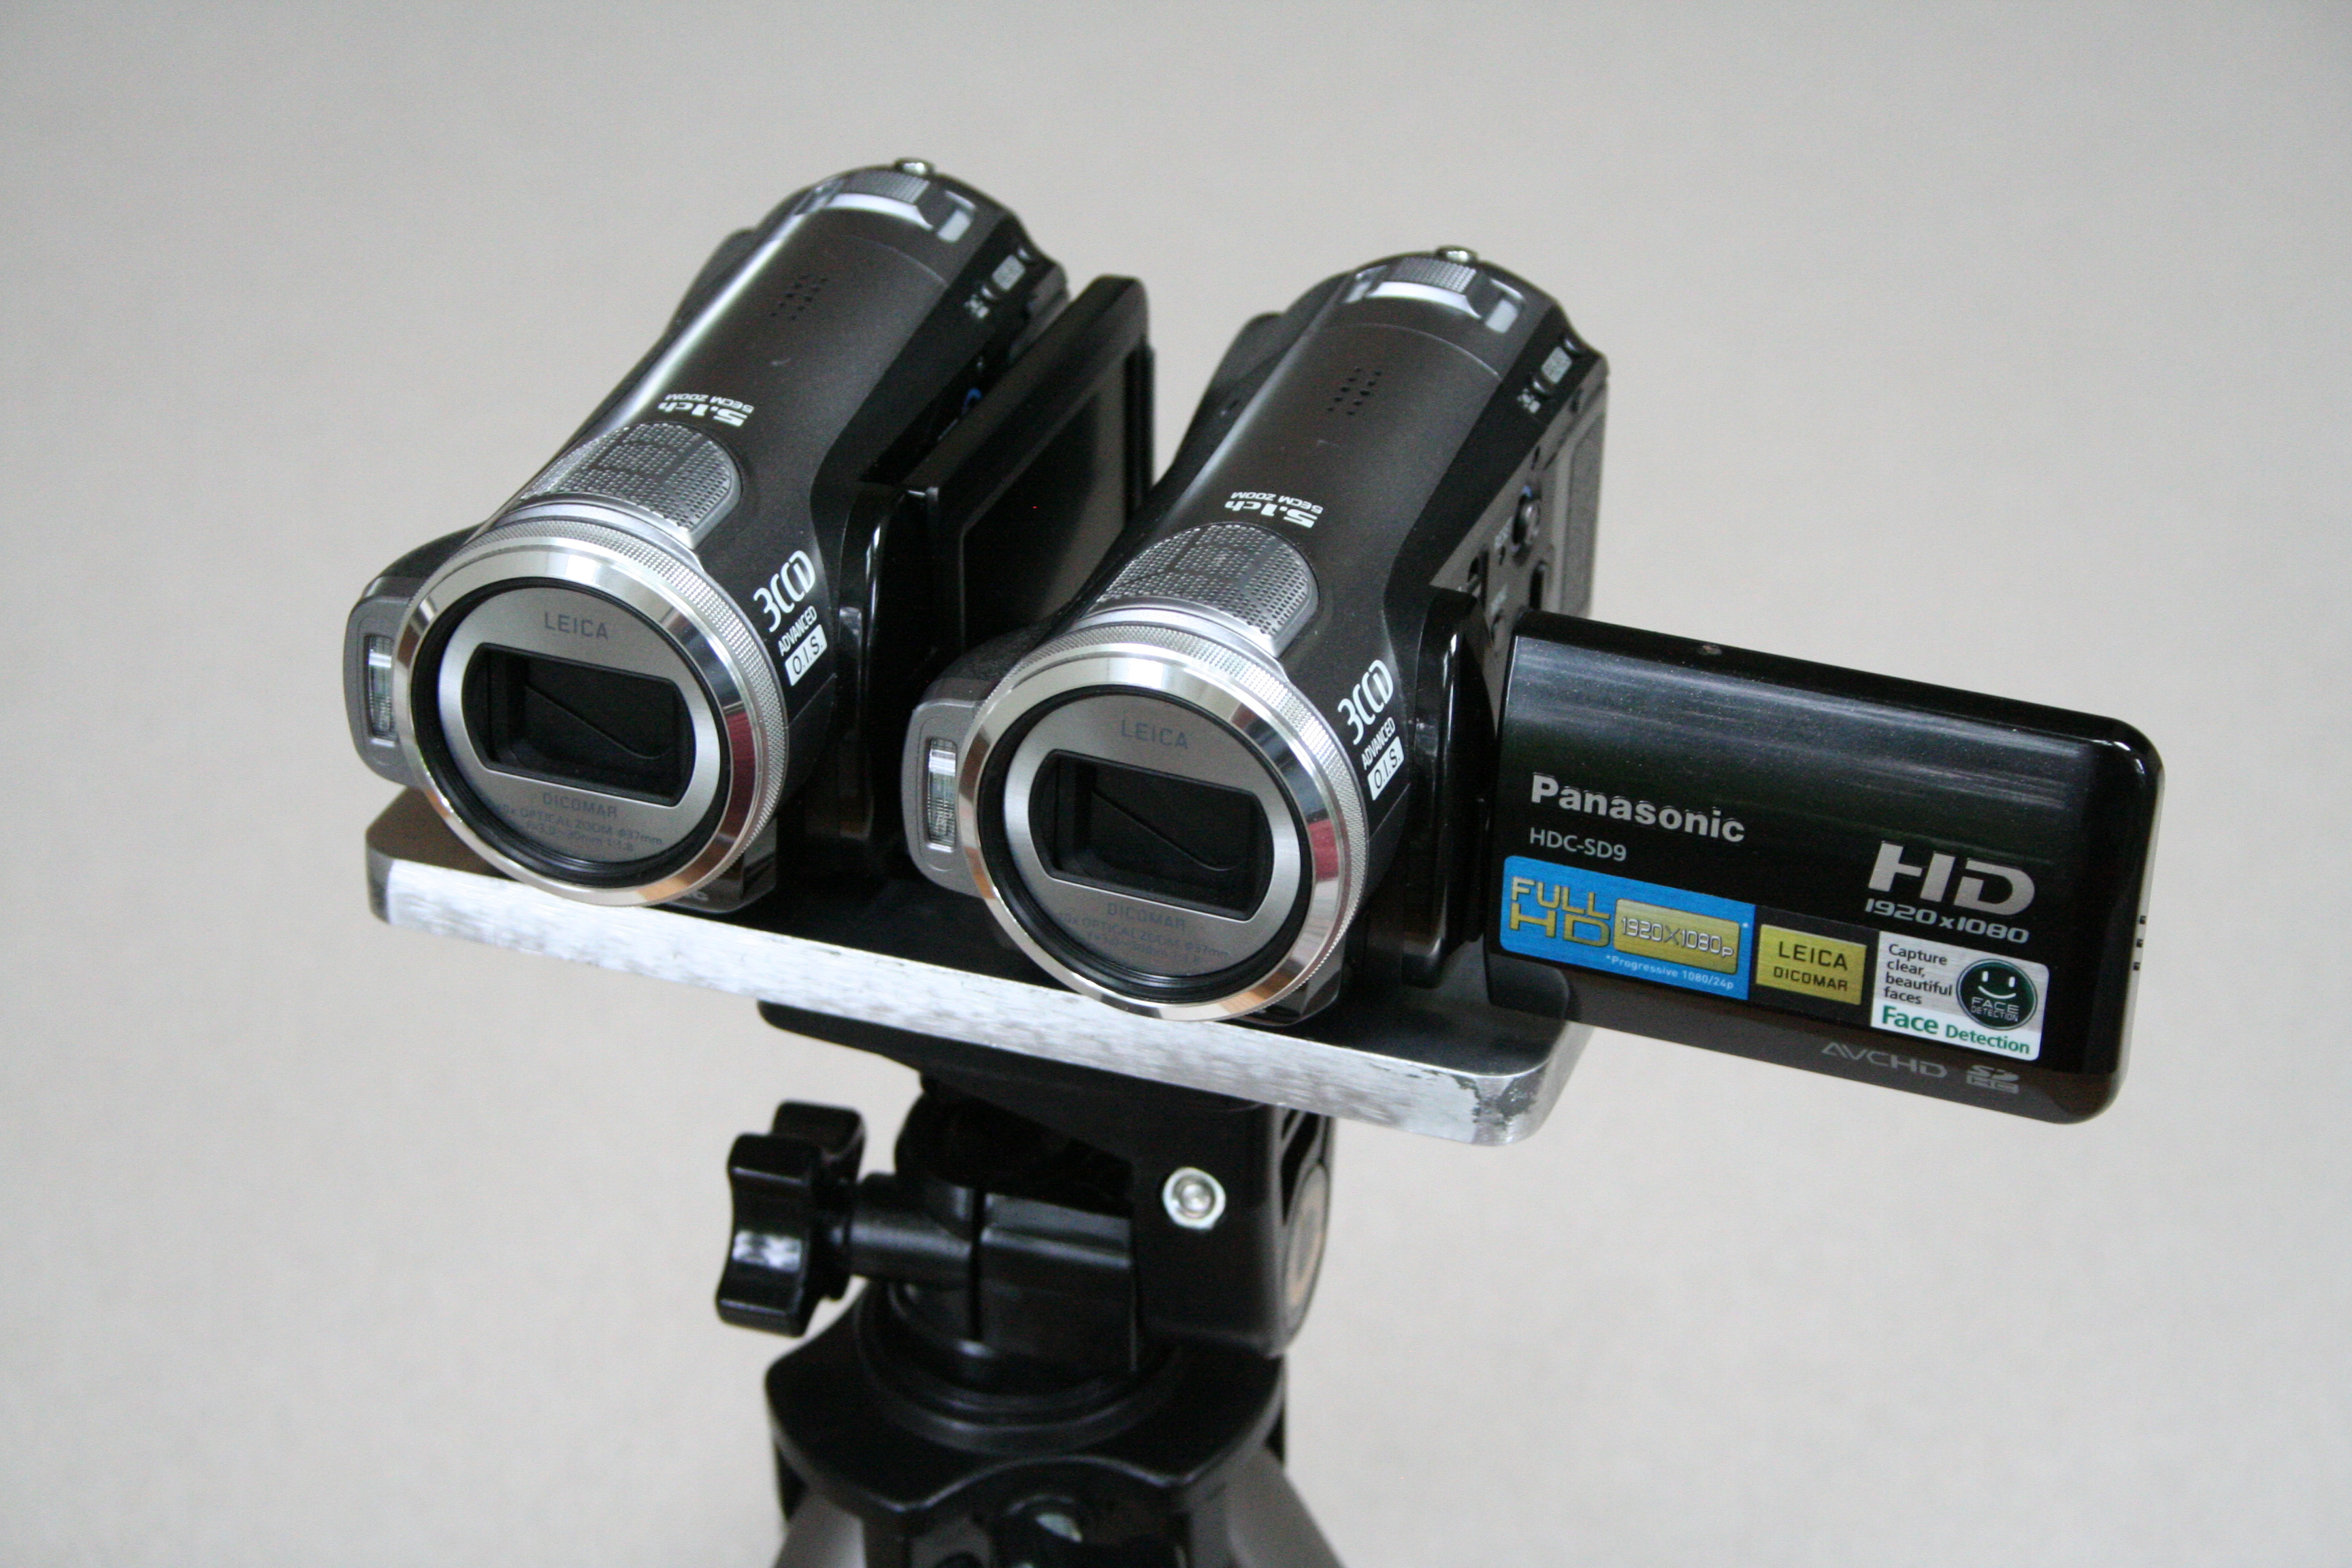
\includegraphics[width=\textwidth]{stereo_rig}
		\caption{Στερεοσκοπική διάταξη}
		\label{fig:stereo_rig}
	\end{subfigure}
\end{figure}

Στην στερεοσκοπική όραση, οι επιπολικές ευθείες είναι \emph{οριζόντιες}, όπως φαίνεται στην εικόνα \ref{fig:stereo_geometry}. Η προϋπόθεση αυτή ικανοποιείται είτε με φυσικό τρόπο, από την κατάλληλη τοποθέτηση στο χώρο των δύο λήψεων σε στερεοσκοπική διάταξη\footnote{Απόδειξη \ref{appendix:stereo_constraint_from_stereo_rig}}, είτε με την εφαρμογή κατάλληλων μετασχηματισμών σε ένα οποιοδήποτε ζεύγος εικόνων, διαδικασία που ονομάζεται ευθυγράμμιση\footnote{\g Απόδειξη \ref{appendix:stereo_constraint_from_rectification}} \e(rectification).\g

Επομένως σε ένα στερεοσκοπικό ζεύγος κάθε τυχαίο σημείο $\mathbf{p_l} = (x,y)$ της αριστερής λήψης:

\begin{itemize}
	\item είτε θα δεν θα βρίσκεται \textbf{πουθενά} στο πέτασμα της δεξιάς (εκτός οπτικού πεδίου της)
	\item είτε θα βρίσκεται στο σημείο $\mathbf{p_r} = (x-d,y)$, όπου $x-d\geq0\Leftrightarrow d \leq x$ \footnote{η περίπτωση όπου $d>x$ αναλογεί στην πρώτη υποπερίπτωση (εκτός οπτικού πεδίου της κάμερας 2)}
\end{itemize}
  
Η τιμή \e d, \g που εκφράζει την οριζόντια μετατόπιση του σημείου ανάμεσα στις δύο λήψεις, ονομάζεται παράλλαξη \e(disparity). \g Με γνωστά τα μεγέθη της στερεοσκοπικής διάταξης $f$, $B$ και της παράλλαξης $d$, ο υπολογισμός του βάθους $Ζ$ του τυχαίου σημείου $p$ είναι άμεσος:

\begin{equation} \label{eq:disp2depth}
	\left. 
		\begin{matrix}
			x_1 = -f\dfrac{X_1}{Z_1} \\
			x_2 = -f\dfrac{X_1 + B}{Z_1}
		\end{matrix}
	\right\} \Rightarrow
	Z_1 = \dfrac{fB}{x_1-x_2} = \dfrac{fB}{d}
\end{equation}

Γεωμετρικά η απόδειξη προκύπτει με κανόνα όμοιων τριγώνων φαίνεται στο σχήμα \ref{fig:disparity_proof}:

$$\dfrac{B}{Z} = \dfrac{(B+x_R)-x_L}{Z-f} \Rightarrow d = x_L - x_r = \dfrac{fB}{Z}$$

\begin{figure}
	\centering
	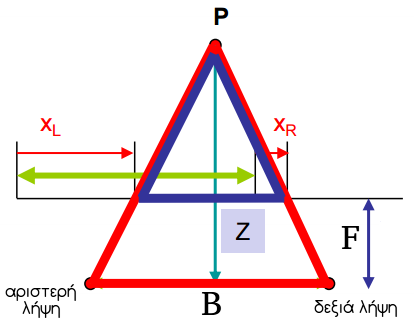
\includegraphics[scale=0.6]{disparity_proof.png}
	\caption{Γεωμετρική απόδειξη σχέσης βάθους και παράλλαξης.}
	\label{fig:disparity_proof}
\end{figure}



\subsection{Πεδίο παραλλάξεων και πεδίο βάθους}

Ο υπολογισμός της παράλλαξης \e d \g κάθε σημείου της εικόνας αναφοράς θα μας οδηγήσει σε έναν νέο πίνακα $D$ όμοιων διαστάσεων με την αρχική εικόνα $D \in \mathbb{R}^{height \times width}$, όπου σε κάθε του θέση θα είναι αποθηκευμένη η πληροφορία παράλλαξης του αντίστοιχου σημείου, όπως φαίνεται στο σχήμα \ref{fig:teddy}. Η παράλλαξη μετράται είτε σε $pixels$ είτε σε $cm$. Επί της ουσίας οι δύο μονάδες μέτρησης είναι ισοδύναμες καθώς η οριζόντια πλευρά του $pixel$ μετράται και αυτή σε $cm$. Στην παρούσα εργασία χρησιμοποιούμε ως μονάδα μέτρησης της παράλλαξης το $pixel$. Το πεδίο τιμών του χάρτη παραλλάξεων είναι το σύνολο $[0,width]$, διότι αν ένα σημείο αναλογεί σε παράλλαξη $> width$ τότε βρίσκεται εκτός οπτικού πεδίου της κάμερας 2.

Χάρτης βάθους \e (depth map) \g είναι ένας πίνακας $depth \in \mathbb{R}^{height \times width}$ που περιέχει την πληροφορία βάθους κάθε σημείου της εικόνας. Κατ' αντιστοιχία, επιλέγουμε ως μονάδα μέτρησης τα $pixels$. Το πεδίο τιμών του χάρτη παραλλάξεων είναι το σύνολο $[\dfrac{f\cdot b}{width},\infty]$, διότι αν ένα σημείο αναλογεί σε βάθος $< \dfrac{f\cdot b}{width}$ τότε βρίσκεται εκτός οπτικού πεδίου της κάμερας 2.

Η μετάβαση από το πεδίο των παραλλάξεων στο πεδίο του βάθους είναι '1-1' και αντιστρέψιμη. Οι δύο αναπαραστάσεις είναι ισοδύναμες.

$$disparity \xleftrightarrow[g^{-1}]{g} depth$$
$$ g:\mathbb{R}^{height \times width} \rightarrow \mathbb{R}^{height \times width} : depth = g(disparity) = \dfrac{fB}{disparity}$$
$$ g^{-1}:\mathbb{R}^{height \times width} \rightarrow \mathbb{R}^{height \times width} : disparity = g^{-1}(depth) = \dfrac{fB}{depth}$$

\begin{figure}
	\centering
	\begin{subfigure}{.32\textwidth}
		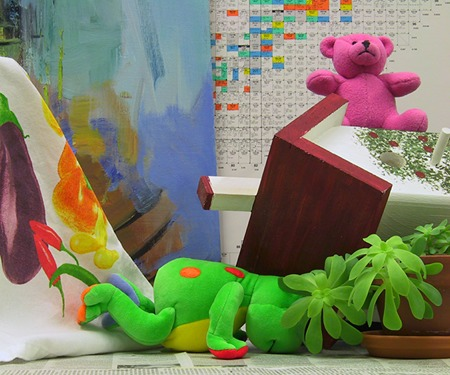
\includegraphics[width=\textwidth]{teddy_im2.jpg}
		\caption{Αριστερή λήψη}
	\end{subfigure}
	\begin{subfigure}{.32\textwidth}
		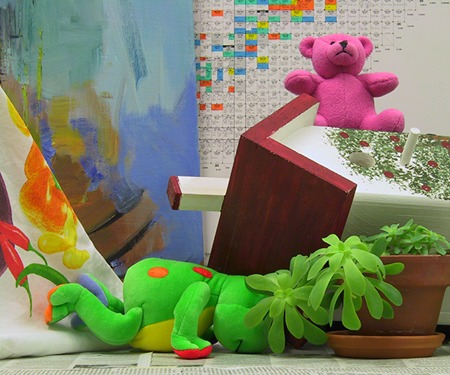
\includegraphics[width=\textwidth]{teddy_im6.jpg}
		\caption{Δεξιά λήψη}
	\end{subfigure}
	\begin{subfigure}{.32\textwidth}
		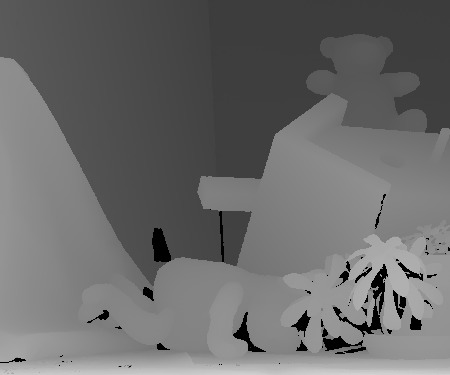
\includegraphics[width=\textwidth]{teddy_disp2.jpg}
		\caption{χάρτης παράλλαξης}
	\end{subfigure}
	\caption{παράδειγμα στερεοσκοπικής λήψης}
	\label{fig:teddy}
\end{figure}

%%%%%%%%%%%%%%%%%%%%%%%%%%%%%%%%%%%%%%%%%%%%%%%%%%%%%%%%%%%%%%%%%%%%%%%%%%%%%%%%%%%%%%%%%%%%%%%%%%%%%%%%%%%%%%%%%%%%%%%%%%%%
%%%%%%%%%%%%%%%%%%%%%%%%%%%%%%%%%%%%%%%%%%%%%%%%%%%%%%%%%%%%%%%%%%%%%%%%%%%%%%%%%%%%%%%%%%%%%%%%%%%%%%%%%%%%%%%%%%%%%%%%%%%%
%%%%%%%%%%%%%%%%%%%%%%%%%%%%%%%%%%%%%%%%%%%%%%%%%%%%%%%%%%%%%%%%%%%%%%%%%%%%%%%%%%%%%%%%%%%%%%%%%%%%%%%%%%%%%%%%%%%%%%%%%%%%

\section{Αρχές και περιορισμοί της στερεοσπικής αντιστοίχησης} \label{sec:stereo_constraints}


Για την διεκπεραίωση της στερεοσκοπικής αντιστοίχησης βασιζόμαστε σε υποθέσεις που οδηγούν σε αντίστοιχους περιορισμούς, κάποιοι εκ των οποίων έχουν καθολική κι άλλοι μερική ισχύ.\cite{pollefeys2004visual} Παραθέτουμε τους βασικότερους:

\begin{enumerate}[label=\textbf{\arabic*.}, ref={\arabic*}]
	\item \label{prop:stereo_contraint} \textbf{Στερεοσκοπικός περιορισμός \e (stereo constraint):} \g Όπως αποδείχθηκε στη σχέση \ref{eq:stereo_constraint}, η αναζήτηση του αντίστοιχου σημείου περιορίζεται αυστηρά και μόνο κατά μήκος της οριζόντιας επιπολικής ευθείας.
	\item \label{prop:disparity_continuity_constraint} \textbf{Περιορισμός συνέχειας/ασυνέχειας παράλλαξης \e (disparity continuity/discontinuity constraint):} \g
	\begin{itemize}
		\item Κατά μήκος συνεχών επιφανειών, οι τιμές της παράλλαξης είναι συνεχείς. Ο περιορισμός αίρεται μόνο στην περίπτωση όπου μια συνεχής επιφάνεια δημιουργεί εσωτερικά "κρυμμένα σημεία".\footnote{"Κρυμμένα σημεία" ονομάζουμε τα σημεία του χώρου που δεν είναι ορατά από μια λήψη.}
		\item Κατά μήκος ασυνεχών επιφανειών, οι τιμές της παράλλαξης είναι ασυνεχείς. Ο περιορισμός αίρεται στην περίπτωση που δύο ασυνεχείς επιφάνειες τυχαίνει να βρίσκονται στο ίδιο βάθος.\footnote{Όπως για παράδειγμα μια επιγραφή σε έναν τοίχο.}
	\end{itemize}
	Επομένως, ασυνέχειες στις τιμές της παράλλαξης συμβαίνουν είτε σε μεταβάσεις από μια επιφάνεια του χώρου σε μια άλλη, είτε αν δημιουργείται εντός μιας επιφάνειας εσωτερικό "κρυμμένο σημείο".
	\item \label{prop:uniqueness_contraint}\textbf{Περιορισμός μοναδικότητας \e (uniqueness constraint):} \g Σε αδιαφανή αντικείμενα, κάθε σημείο της μίας λήψης έχει το πολύ ένα σημείο αντιστοίχησης στην έτερη λήψη. Πιο συγκεκριμένα, ένα και μοναδικό, εάν είναι ορατό από την έτερη λήψη, και κανένα εάν δεν είναι ορατό.\footnote{η περίπτωση αυτή ονομάζεται απόκρυψη.} Έστω $\mathbf{p_1} \in I^{L}$, τότε 
	\[
	\mathbf{p_1}\xrightarrow{corresponds} \left\{
		\begin{array}{ll}
			\emptyset,\: \text{απόκρυψη} \\
            	\mathbf{p_2} \in I^{R},\: \text{αλλιώς}  \\
         \end{array}
          						\right.
    \]
    Στις περιοχές που είναι ορατές και από τις δύο λήψεις η παραπάνω σχέση γίνεται "1-1". Μπορούμε δηλαδή να αντιστοιχήσουμε μια αντιστρεπτή συνάρτηση $g$ μετάβασης ανάμεσα στα αντίστοιχα σημεία.
	\[
	p_1 \xLeftrightarrow[g^{-1}]{g} p_2
	\]
	Παραστατική απεικόνιση του περιορισμού μοναδικότητας παρουσιάζεται στο σχήμα \ref{fig:uniqueness_constraint}
	Ο περιορισμός παραβιάζεται μόνο σε σπάνιες περιπτώσεις διαφανών αντικειμένων, όπου δύο σημεία του τρισδιάστατου χώρου μπορεί να αποτυπώνονται ταυτόχρονα στο ίδιο σημείο του ενός πετάσματος και σε δύο διακριτά σημεία του έτερου. \ref{fig:transparent_object}
	\item \label{prop:ordering_contraint} \textbf{Περιορισμός διάταξης παραλλάξεων \e (ordering constraint):} \g Το σύνολο των σημείων που απαρτίζουν το είδωλο της επιφάνειας ενός αδιαφανούς αντικειμένου της τρισδιάστατης σκηνής, είναι διατεταγμένα κατά τον ίδιο τρόπο στις δύο λήψεις. Πρακτικά, ένα σημείο της επιφάνειες που αποτυπώθηκε πιο αριστερά από ένα άλλο στο ένα πέτασμα, δεν μπορεί να αποτυπωθεί αντίστροφα (πιο δεξιά) στο άλλο πέτασμα. \ref{fig:ordering_constraint_success} Ο ισχυρισμός καταρρέει αν μεταβούμε από την επιφάνεια ενός αντικειμένου σε αυτή ενός άλλου. \ref{fig:ordering_constraint_failure} Την περιοχή του χώρου εντός της οποίας αίρεται ο περιορισμός διάταξης, την αποκαλούμε "απαγορευμένη ζώνη" \e (forbidden zone). \g \ref{fig:forbidden_zone}
	\item \label{prop:stereo_constancy} \textbf{Σταθερότητα φωτισμού \e (color constancy):} \g Ο φωτισμός και ο χρωματισμός κάθε σημείου μιας σκηνής παραμένει αμετάβλητος σε κάθε θέση παρατήρησης της σκηνής. Ο ισχυρισμός αυτός ισχύει για τις λαμπερτιανές επιφάνειες που προκαλούν διάχυση, αναιρείται όμως όταν η σκηνή περιλαμβάνει μη-λαμπερτιανές (λείες ή διαφανείς επιφάνειες) που προκαλούν φαινόμενα κατοπτρικής ανάκλασης και διάθλασης.
	\item \label{prop:disparity_limit} \textbf{Όριο μέγιστης παράλλαξης \e (disparity limit):} \g Η μέγιστη δυνατή παράλλαξη του τυχαίου σημείου $p_1 = (x,y)$ της αριστερής κάμερας είναι η $d = x$, τιμή μεταβλητή ανάλογα με την τετμημένη του μελετούμενου σημείου. Σε κάθε περίπτωση η πιθανή παράλλαξη δεν μπορεί να υπερβαίνει το πλάτος της εικόνας $d \in [0,width]$. Πολλές φορές θέτουμε ένα, σχετικά αυθαίρετο, αυστηρότερο όριο ως μέγιστη παράλλαξη $d_{max}$, όταν δεν μας ενδιαφέρει ο ακριβής υπολογισμός του βάθους αντικειμένων που βρίσκονται πιο κοντά από το όριο αυτό. Το επίπεδο $Z = Z_{min}$ θέτει έναν κόφτη πέρα του οποίου όλα τα αντικείμενα χαρακτηρίζονται ως "πολύ κοντινά". Η σύμβαση του μέγιστου ορίου παράλλαξης έχει το σημαντικό πλεονέκτημα της μείωσης της υπολογιστικής πολυπλοκότητας.
\end{enumerate}

Θα μπορούσαμε να ομαδοποιήσουμε τους περιορισμούς 2, 3, 4 και 5 σε μια πιο ενιαία και ασαφή περιγραφή, αυτήν της "ομοιότητας γειτονιάς" \e(patches similarity). \label{prop:patches_similarity} \g Η "ομοιότητα γειτονιάς", εγκολπώνοντας τους παραπάνω περιορισμούς, υποθέτει ότι μια δεδομένη περιοχή της τρισδιάστατης σκηνής θα έχει \textit{παρόμοια} προβολή (σχήμα, χρώμα, μορφή, υφή) στα πετάσματα των δύο καμερών. Με δεδομένη αυτή την υπόθεση, θα αναζητήσουμε ακολούθως μετρικές ομοιότητας ώστε να αξιολογήσουμε την ομοιότητα περιοχών γύρω από τα σημεία ενδιαφέροντος και να "ταιριάξουμε" τα πλέον όμοια, δημιουργώντας τον ζητούμενο πίνακα παράλλαξης.

\begin{figure}
	\centering
	\begin{subfigure}{.6\textwidth}
		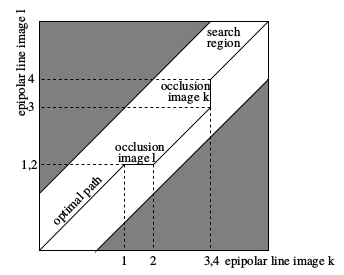
\includegraphics[width=\textwidth]{uniqueness1.png}
	\end{subfigure}
	\begin{subfigure}{.6\textwidth}
		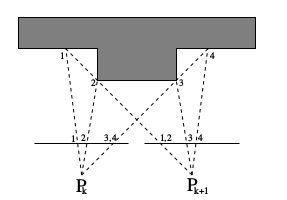
\includegraphics[width=\textwidth]{uniqueness2.png}
	\end{subfigure}
	\caption{Περιορισμός μοναδικότητας. Στο γράφημα ο οριζόντιος άξονας είναι η επιπολική γραμμή της αριστερής λήψης, ενώ ο κάθετος της δεξιάς. Παρατηρούμε ότι στις περιοχές που δεν υφίσταται απόκρυψη, δηλαδή μέχρι το σημείο 1, ανάμεσα στα σημεία 2,3 και μετά το σημείο 4, η σχέση που συνδέει τα αντίστοιχα σημεία είναι "1-1". Αντιθέτως στα σημεία που υπάρχει απόκρυψη για κάποια από τις δύο λήψεις, δηλαδή στις περιοχές ανάμεσα στα σημεία 1,2 και 3,4, η σχέση δεν είναι αντιστρεπτή.}
	\label{fig:uniqueness_constraint}
\end{figure}

\begin{figure}
	\centering
	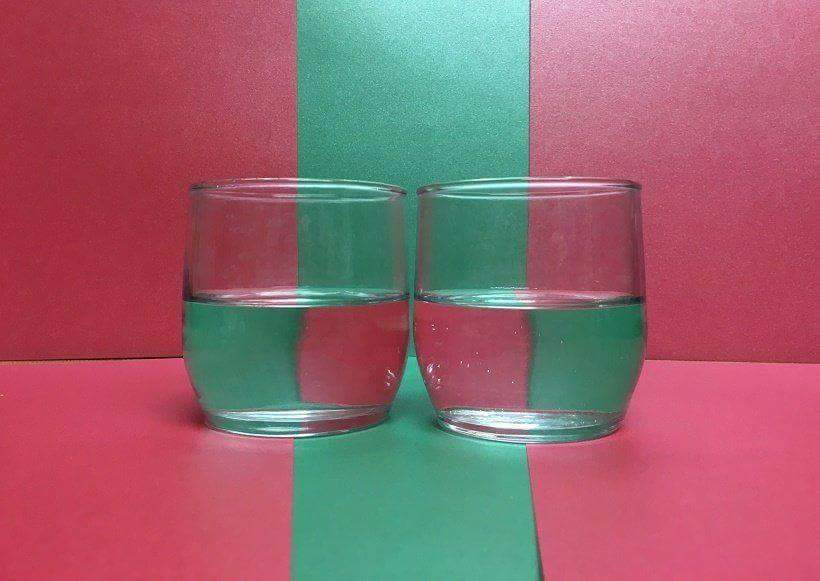
\includegraphics[width=0.5\textwidth]{transparent_object.jpg}
	\caption{Τα διάφανα αντικείμενα παραβιάζουν τον περιορισμό μοναδικότητας.}
	\label{fig:transparent_object}
\end{figure}

\begin{figure}
	\centering
	\begin{subfigure}{.49\textwidth}
		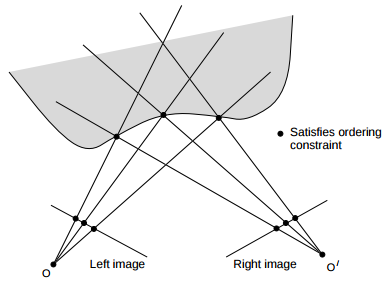
\includegraphics[width=\textwidth]{ordering_constraint.png}
		\caption{Περιορισμός διάταξης σε συνεχείς αδιαφανείς επιφάνειες}
		\label{fig:ordering_constraint_success}
	\end{subfigure}
	\begin{subfigure}{.49\textwidth}
		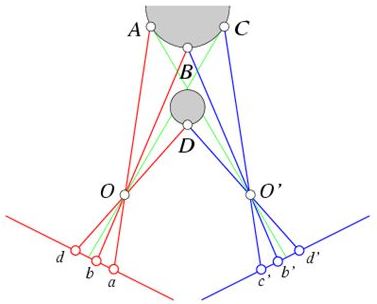
\includegraphics[width=\textwidth]{ordering_constraint_failure.png}
		\caption{Ο περιορισμός διάταξης αίρεται σε ασυνεχείς επιφάνειες}
		\label{fig:ordering_constraint_failure}
	\end{subfigure}
	\begin{subfigure}{.49\textwidth}
		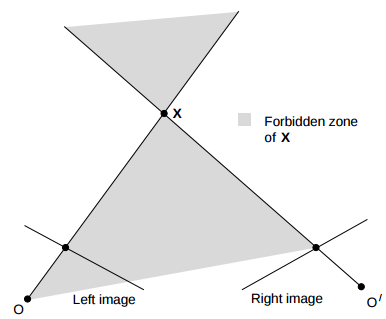
\includegraphics[width=\textwidth]{forbidden_zone.png}
		\caption{Απαγορευμένη περιοχή: οποιοδήποτε σημείο εντός της σκιασμένης περιοχής αναιρεί τον περιορισμό διάταξης παραλλάξεων}
		\label{fig:forbidden_zone}
	\end{subfigure}
	\caption{Περιορισμός διάταξης παραλλάξεων}
	\label{fig:ordering_constraint}
\end{figure}

%%%%%%%%%%%%%%%%%%%%%%%%%%%%%%%%%%%%%%%%%%%%%%%%%%%%%%%%%%%%%%%%%%%%%%%%%%%%%%%%%%%
%%%%%%%%%%%%%%%%%%%%%%%%%%%%%%%%%%%%%%%%%%%%%%%%%%%%%%%%%%%%%%%%%%%%%%%%%%%%%%%%%%%

\section{Μελέτη φαινομένων που αμφισβητούν τους περιορισμούς της στερεοσπικής αντιστοίχησης} \label{sec:stereo_constraints_violation}

Η υπόθεση της "ομοιότητας γειτονιάς" δεν έχει καθολική ισχύ. Εξ' ορισμού η προοπτική προβολή είναι μια πράξη μετασχηματισμού που αλλοιώνει το σχήμα του προβαλλόμενου αντικειμένου. Οι διαφορετικές θέσεις λήψης δημιουργούν διαφορετικά προβαλλόμενα είδωλα. Για αυτόν τον λόγο διαχωρίζουμε τα προβλήματα της στερεοσκοπικής αντιστοίχησης σε δύο μεγάλες κατηγορίες, στα προβλήματα μικρής και μεγάλης απόστασης βάσης \e (small and wide baseline stereo rig problems). \g Η βάση αναφέρεται στην οριζόντια απόσταση \e B (baseline) \g των δύο λήψεων. Στα προβλήματα μεγάλης απόστασης βάσης τα δύο είδωλα του ίδιου τρισδιάστατου αντικειμένου αποκλίνουν έντονα σε σχήμα, χρώμα και μορφή. Η απόκλιση οξύνεται κατ' αναλογία της αύξησης του μεγέθους \e B. \g \ref{fig:wide_baseline}
Στα προβλήματα μικρής απόστασης βάσης, που μας απασχολούν στην παρούσα εργασία, το φαινόμενο της σχηματικής, χρωματικής και μορφολογικής αλλοίωσης είναι αρκετά μειωμένο, όπως παρατηρούμε και στις εικόνες \ref{fig:small_baseline} \ref{fig:teddy}, χωρίς βέβαια να εξαφανίζεται πλήρως \ref{fig:perspective_transformation}. Επομένως είναι αρκετά βάσιμο να στηριχτούμε στην "ομοιότητα γειτονιάς" σε ένα ικανοποιητικό υποσύνολο των περιοχών της εικόνας. Σε συγκεκριμένες θέσεις παρατηρούνται φαινόμενα που αναιρούν ευθέως την παραπάνω υπόθεση, και κατ' επέκταση τις τέσσερις βασικές υποθέσεις που έχει στηριχτεί. Παρακάτω παραθέτουμε μια συνοπτική ανάλυση των φαινομένων αυτών:

\begin{enumerate}[label=\textbf{\arabic*.}, ref={\arabic*}]
	\item \label{prop:occlusions} \textbf{Αποκρύψεις \e(Occlusions):\g} Η έστω και μικρή μετατόπιση στη γωνία θέασης δημιουργεί περιοχές του \e 3D \g χώρου που είναι ορατές μόνο από τη μία εκ των δύο λήψεων, όπως παρατηρούμε στο σχήμα \ref{fig:occlusion}. Οι περιοχές αυτές εντοπίζονται συνήθως σε ασυνέχειες βάθους, δηλαδή σε σημεία που μεταβαίνουμε από ένα αντικείμενο σε ένα άλλο και παραβιάζουν ολοκληρωτικά την υπόθεση της "ομοιότητας γειτονιάς" \ref{fig:occlusion1}. Στις περιοχές αυτές πρέπει να δοθούν τιμές παράλλαξης εντός του διαστήματος τιμών $[D_L, D_R]$, όπου $D_L, D_R$ οι τιμές παράλλαξης των σημείων που βρίσκονται εκατέρωθεν της κρυμμένης περιοχής. Βέλτιστα η μεταβολή των τιμών παράλλαξης εντός της κρυμμένης περιοχής πρέπει να ακολουθεί μια γραμμική μεταβολή από το $D_L$ στο $D_R$, δηλαδή $d = D_L + (D_R - D_L)\dfrac{j - j_L}{j_R - j_L}$, όπου $j$ συμβολίζει την οριζόντια θέση και $D$ την τιμή της παράλλαξης.

	\item \label{prop:foreshortening_effect}\textbf{Φαινόμενο αυξομείωσης αποστάσεων και εμβαδών \e(Foreshortening effect):\g} Η προοπτική προβολή δεν κρατάει αναλλοίωτες τις αποστάσεις και τα εμβαδά. Το φαινόμενο της αυξομείωσης δημιουργεί διπλό πρόβλημα. Αφενός παραβιάζει την υπόθεση "ομοιότητας γειτονιάς", αφετέρου καθιστά και την αντιστοίχηση μη αντιστρεπτή καθώς $n \: pixels$ της μιας λήψης αντιστοιχούνται σε $m\neq n \: pixels$ της έτερης, παρ' ότι το αντικείμενο είναι \emph{απόλυτα ορατό και από τις δύο λήψεις}. \ref{fig:foreshortening}
	
	\item \label{prop:photometric_variations}\textbf{Αλλοιώσεις φωτισμού}: Ο όρος φωτισμός περιγράφει την διαδικασία υπολογισμού της έντασης της φωτεινής ακτινοβολίας που προσλαμβάνει ο θεατής, που στην περίπτωσή μας είναι οι στερεοσκοπικές κάμερες. Η φωτεινή ακτινοβολία, δηλαδή το εγκάρσιο κύμα του ορατού φωτός που προσπίπτει στο πέτασμα της κάμερας, μπορεί να έχει προέλθει από τέσσερα φυσικά φαινόμενα: αυτοφωτισμό, ανάκλαση, διάθλαση και διάχυση. Εκ των τεσσάρων αυτών φαινομένων, η κατοπτρική ανάκλαση και η διάθλαση δημιουργούν φωτισμό που διαφέρει ανάλογα με την θέση του θεατή. Το φαινόμενο αυτό ονομάζεται μη λαμπερτιανό φαινόμενο φωτισμού \e(non-lambertian lighting effect)\g και οι επιφάνειες που το προκαλούν ονομάζονται μη λαμπερτιανές \e(non-lambertian) \g επιφάνειες. Παραθέτουμε επιλεκτικά κάποιες περιπτώσεις:
	\begin{enumerate}
		\item \textbf{Κατοπτρικές ανακλάσεις:} Σε αυτήν την περίπτωση μια μη λαμπερτιανή επιφάνεια (π.χ. καθρέπτης) αποτυπώνει στο πέτασμα της κάμερας το είδωλο ενός τρίτου αντικείμενου το οποίο κατοπτρίζει. Το είδωλο του τρίτου αντικειμένου, που τελικά αποτυπώνεται στον φακό, υφίσταται μεγάλες αλλοιώσεις ακόμα και σε μικρές μεταβολές της θέσης του θεατή. \ref{fig:specular_reflection}
Το παραπάνω πολύ δύσκολα αντιμετωπίσιμο φαινόμενο είναι σχετικά σπάνιο. Μια πιο συνηθισμένη εκδοχή του είναι ο εστιασμένος κατοπτρισμός μιας φωτεινής πηγής, που δημιουργεί αλλοιωμένη φωτεινότητα στα προβαλλόμενα είδωλα. \ref{fig:specularity}.
		\item \textbf{Φωτομετρικές αποκλίσεις \e(photometric variations): \g} Συνήθως δεν προκαλεί ολική αλλοίωση στα δύο είδωλα, αλλά μια απόκλιση κυρίως στη φωτεινότητα και στο χρώμα. Αν το φαινόμενο είναι πολύ έντονο, η μεγάλη απόκλιση στη διαφορά φωτεινότητας μπορεί να κάνει ακατάληπτο το σχήμα του ειδώλου \ref{fig:photometric_variation}. Έντονες φωτομετρικές αποκλίσεις μεταξύ των δύο λήψεων προκαλούν συχνά οι σκιάσεις.
	\end{enumerate}
\end{enumerate}

Υπάρχουν επίσης περιπτώσεις όπου ενώ η "ομοιότητα γειτονιάς" τηρείται, δημιουργούνται ιδιαίτερα μοτίβα που δημιουργούν σύγχυση σε μια απλή μετρική ομοιότητας:
\begin{enumerate}[label=\textbf{\arabic*.}, ref={\arabic*}]
	\item \label{prop:repetitice_patterns}\textbf{Επαναλαμβανόμενα μοτίβα, δομές και υφές\e(repetitive patterns, structures and textures):\g} αν το φωτογραφιζόμενο τοπίο εμφανίζει επαναλαμβανόμενα μοτίβα (όπως βιβλία σε μια βιβλιοθήκη, ρίγες μιας ζέβρας ή μια σκακιέρα) ή επαναλαμβανόμενες υφές (όπως μια εικόνα από πολλά τριαντάφυλλα) τότε έντονη "ομοιότητα γειτονιάς" εμφανίζεται σε περισσότερα από ένα σημεία στην έτερη εικόνα, προκαλώντας αδυναμία επιλογής της καταλληλότερης περιοχής για αντιστοίχηση. Μια μετρική ομοιότητας γειτονιών εμφανίζει σε αυτήν την περίπτωση πολλά τοπικά μέγιστα. \ref{fig:repetitive}
	\item \label{prop:uniform_regions}\textbf{Μεγάλες ομοιόμορφες περιοχές \e(uniform regions):\g} αν το εικονιζόμενο τοπίο χαρακτηρίζεται από μεγάλες ομοιόμορφες περιοχές, όπως για παράδειγμα ο ουρανός, ο τοίχος μιας πολυκατοικίας και πολλά άλλα, η "ομοιότητα γειτονιάς" παραμένει παρόμοια (κατά περιπτώσεις και τελείως ίδια) σε μεγάλο εύρος διαφορετικών παραλλάξεων. Η μετρική ομοιότητας μένει για πολλές διαδοχικές τιμές παράλλαξης κοντά στο ολικό μέγιστο.
\end{enumerate}

Τέλος, υπάρχουν προβλήματα που δημιουργούνται λόγω θορύβου που προστίθεται κατά την λήψη της φωτογραφίας από το στερεοσκοπικό ζεύγος, όπως για παράδειγμα στην διαφορετική εστίαση όπου δημιουργείται θόλωμα \e(blur)\g κατά δυαδικό τρόπο σε κάθε λήψη δυσκολεύοντας την ανίχνευση της ομοιότητας. \ref{fig:different_focus}

\begin{figure}
	\centering
	\begin{subfigure}{.49\textwidth}
		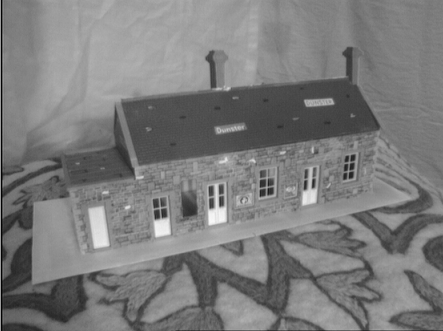
\includegraphics[width=\textwidth, height=0.55\textwidth]{wide_baseline_1_left.png}
		\caption{Αριστερή λήψη}
	\end{subfigure}
	\begin{subfigure}{.49\textwidth}
		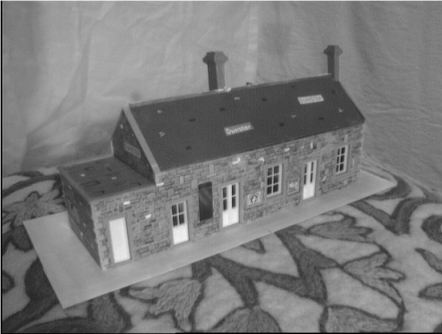
\includegraphics[width=\textwidth, height=0.55\textwidth]{wide_baseline_1_right.png}
		\caption{Δεξιά λήψη}
	\end{subfigure}
	\caption{Στερεοσκοπική λήψη μεγάλης απόστασης βάσης}
	\label{fig:wide_baseline}
\end{figure}

\begin{figure}
	\centering
	\begin{subfigure}{.49\textwidth}
		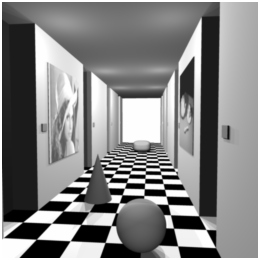
\includegraphics[width=\textwidth, height=0.55\textwidth]{small_baseline_1_left.png}
		\caption{Αριστερή λήψη}
	\end{subfigure}
	\begin{subfigure}{.49\textwidth}
		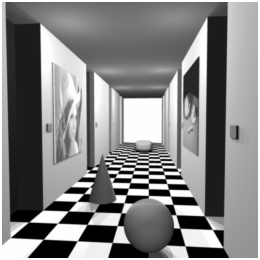
\includegraphics[width=\textwidth, height=0.55\textwidth]{small_baseline_1_right.png}
		\caption{Δεξιά λήψη}
	\end{subfigure}
	\caption{Στερεοσκοπική λήψη μικρής απόστασης βάσης}
	\label{fig:small_baseline}
\end{figure}

\begin{figure}
	\centering
	\begin{subfigure}{.49\textwidth}
		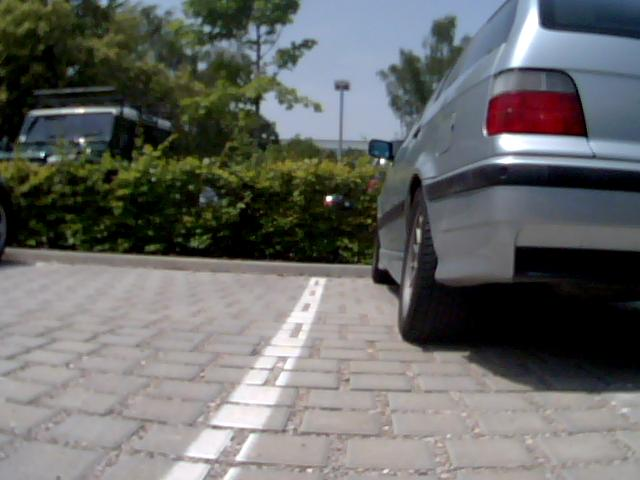
\includegraphics[width=\textwidth, height=0.55\textwidth]{perspective_transformation_l.png}
		\caption{Αριστερή λήψη}
	\end{subfigure}
	\begin{subfigure}{.49\textwidth}
		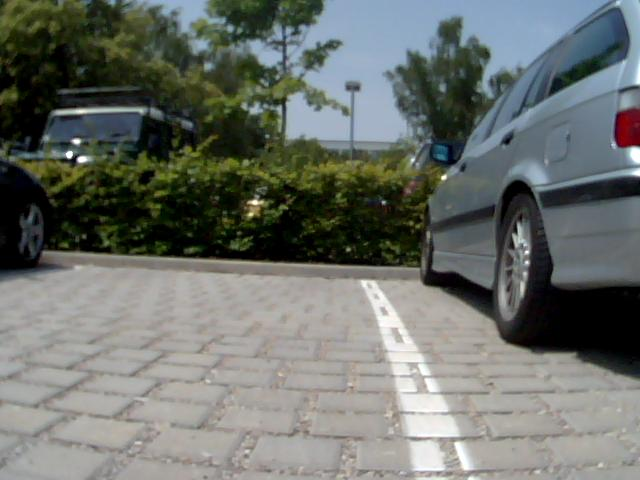
\includegraphics[width=\textwidth, height=0.55\textwidth]{perspective_transformation_r.png}
		\caption{Δεξιά λήψη}
	\end{subfigure}
	
	\begin{subfigure}{.49\textwidth}
		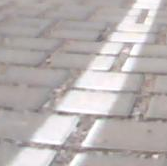
\includegraphics[width=\textwidth, height=0.55\textwidth]{perspective_transformation_l_crop.png}
		\caption{Αριστερή λήψη}
	\end{subfigure}
	\begin{subfigure}{.49\textwidth}
		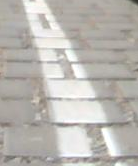
\includegraphics[width=\textwidth, height=0.55\textwidth]{perspective_transformation_r_crop.png}
		\caption{Δεξιά λήψη}
	\end{subfigure}
	\caption{Αλλοίωση των απεικονιζόμενων σχημάτων λόγω προοπτικής προβολής. Πηγή: \citep{TUMLesson}}
	\label{fig:perspective_transformation}
\end{figure}

\begin{figure}
	\centering
	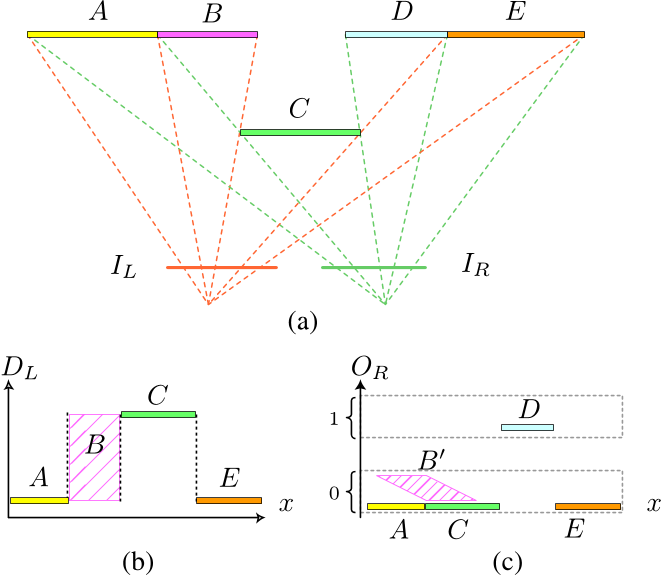
\includegraphics[width=0.8\textwidth]{occlusion_image.png}
	\caption{Ανάλυση φαινομένου απόκρυψης. (a) Στερεοσκοπικό ζεύγος εικόνων $I^L, I^R$ που αποτυπώνει μια σκηνή που περιλαμβάνει τα αντικείμενα \e A, B, C, D, E \g (b) Ο χάρτης παράλλαξης της αριστερής εικόνας. Παρατηρούμε ότι η παράλλαξη του αντικειμένου \e B \g είναι απροσδιόριστη λόγω απόκρυψης (δεν υπάρχει το είδωλό του στην έτερη λήψη). Υποχρεωτικά θα αντιστοιχηθεί είτε με το αντικείμενο \e A \g, είτε με το \e C \g, είτε θα επιμεριστεί σε δύο κομμάτια όπου αναλόγως θα αντιστοιχηθούν σε \e A \g και \e C \g. Γενικά, το αντικείμενο \e B \g θα λάβει τιμή παράλλαξης εντός του πεδίου $[D_A, D_C]$ (γ) Ο χάρτης απόκρυψης της δεξιάς εικόνας. Για την δεξιά εικόνα, το αντικείμενο \e D \g βρίσκεται σε απόκρυψη και όμοια με το (b) θα αντιστοιχηθεί είτε στο \e C \g είτε στο \e E \g.}
	\label{fig:occlusion}
\end{figure}

\begin{figure}
	\centering
	\begin{subfigure}{.49\textwidth}
		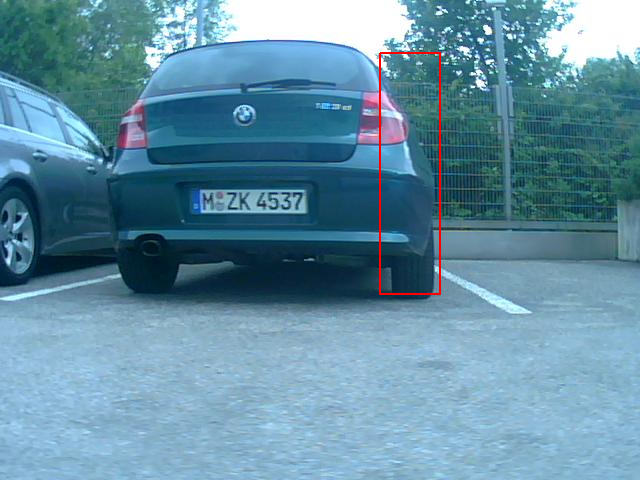
\includegraphics[width=\textwidth, height=0.55\textwidth]{occlusion_1_l.png}
		\caption{Αριστερή λήψη}
	\end{subfigure}
	\begin{subfigure}{.49\textwidth}
		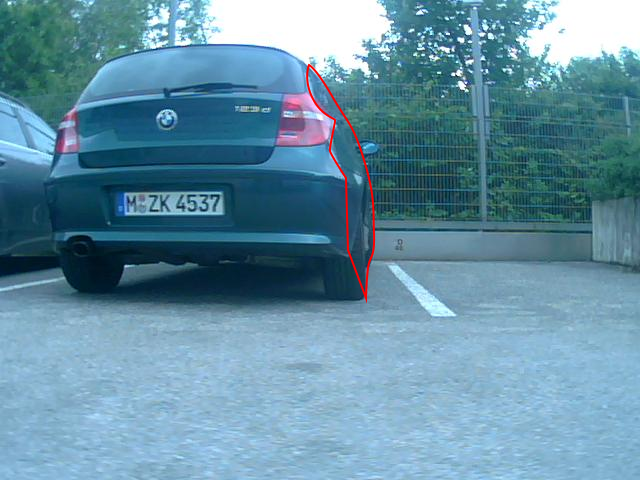
\includegraphics[width=\textwidth, height=0.55\textwidth]{occlusion_1_r.png}
		\caption{Δεξιά λήψη}
	\end{subfigure}
	
	\begin{subfigure}{.49\textwidth}
		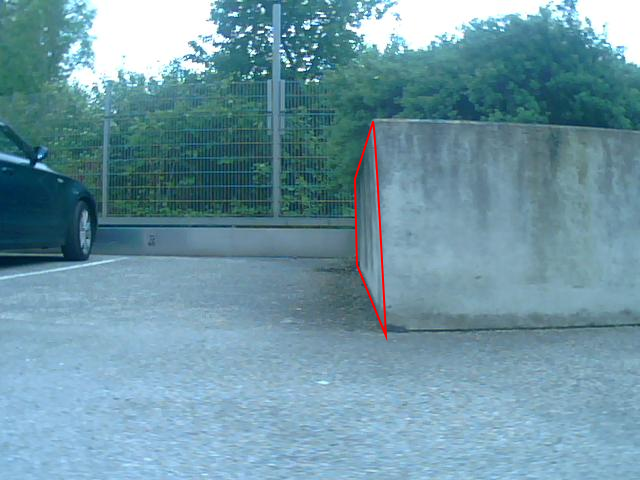
\includegraphics[width=\textwidth, height=0.55\textwidth]{occlusion_2_l.png}
		\caption{Αριστερή λήψη}
	\end{subfigure}
	\begin{subfigure}{.49\textwidth}
		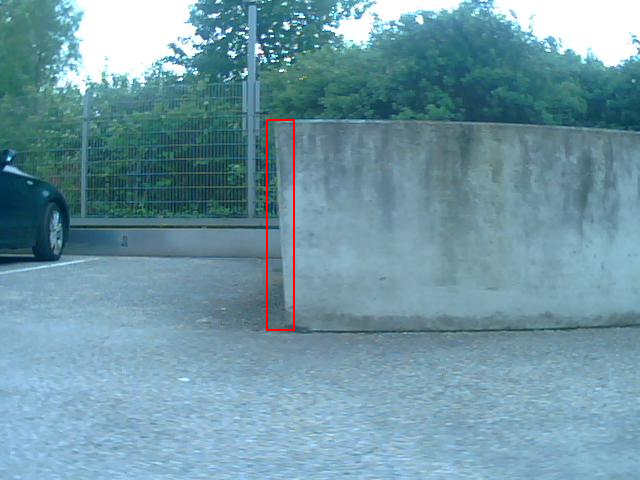
\includegraphics[width=\textwidth, height=0.55\textwidth]{occlusion_2_r.png}
		\caption{Δεξιά λήψη}
	\end{subfigure}
	\caption{Φαινόμενο απόκρυψης. Πηγή: \citep{TUMLesson}}
	\label{fig:occlusion1}
\end{figure}

\begin{figure}
	\centering
	\begin{subfigure}{.49\textwidth}
		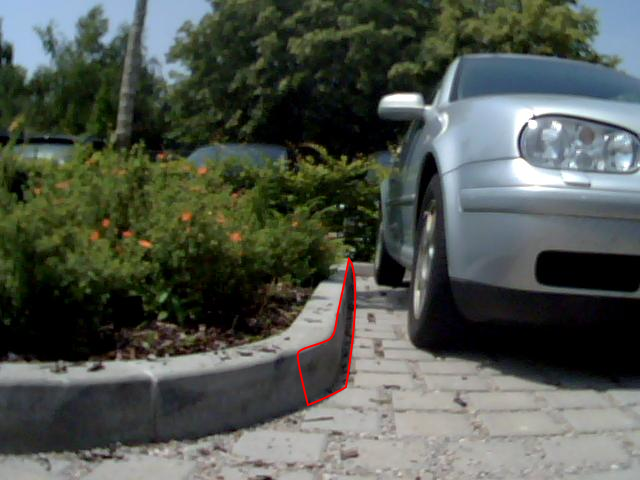
\includegraphics[width=\textwidth, height=0.55\textwidth]{foreshortening_l.png}
		\caption{Αριστερή λήψη}
	\end{subfigure}
	\begin{subfigure}{.49\textwidth}
		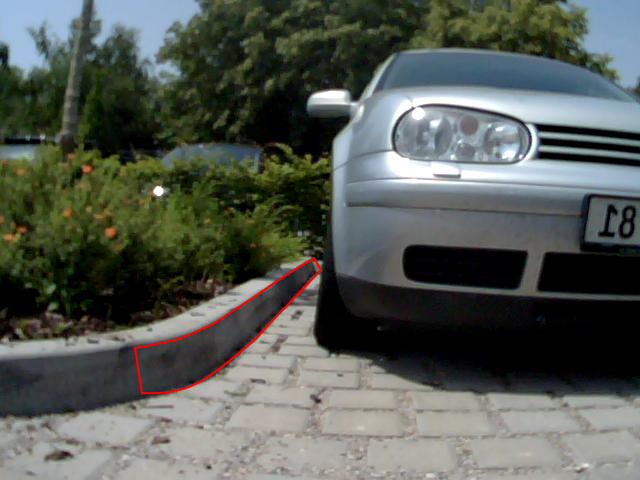
\includegraphics[width=\textwidth, height=0.55\textwidth]{foreshortening_r.png}
		\caption{Δεξιά λήψη}
	\end{subfigure}
	\caption{Φαινόμενο αυξομείωσης αποστάσεων και εμβαδών. Πηγή: \citep{TUMLesson}}
	\label{fig:foreshortening}
\end{figure}

\begin{figure}
	\centering
	\begin{subfigure}{.49\textwidth}
		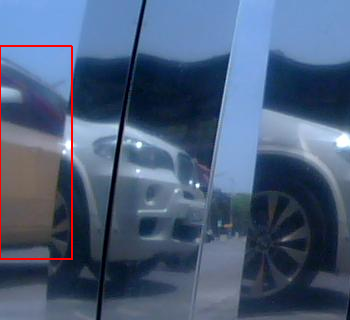
\includegraphics[width=\textwidth, height=0.55\textwidth]{specular_reflection_intense_l.png}
		\caption{Αριστερή λήψη}
	\end{subfigure}
	\begin{subfigure}{.49\textwidth}
		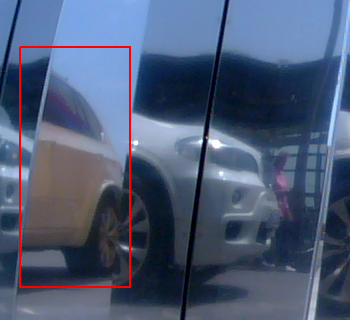
\includegraphics[width=\textwidth, height=0.55\textwidth]{specular_reflection_intense_r.png}
		\caption{Δεξιά λήψη}
	\end{subfigure}
	
	\begin{subfigure}{.49\textwidth}
		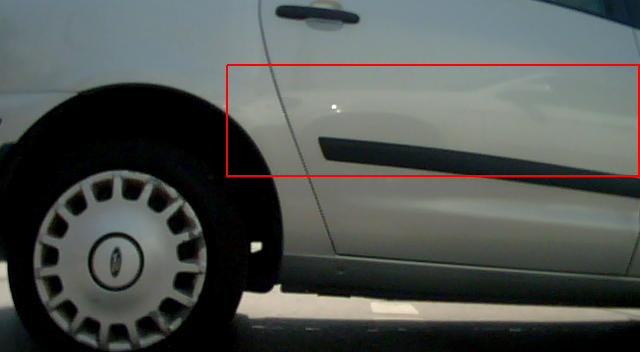
\includegraphics[width=\textwidth, height=0.55\textwidth]{specular_reflection_mild_l.png}
		\caption{Αριστερή λήψη}
	\end{subfigure}
	\begin{subfigure}{.49\textwidth}
		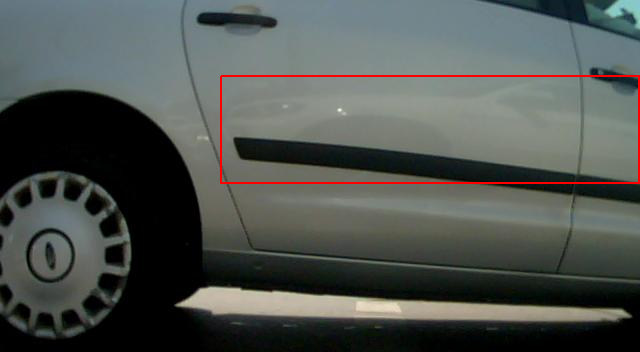
\includegraphics[width=\textwidth, height=0.55\textwidth]{specular_reflection_mild_r.png}
		\caption{Δεξιά λήψη}
	\end{subfigure}
	\caption{Φαινόμενο κατοπτρικής ανάκλασης τρίτου αντικειμένου. Πηγή: \citep{TUMLesson}}
	\label{fig:specular_reflection}
\end{figure}

\begin{figure}
	\centering
	\begin{subfigure}{.49\textwidth}
		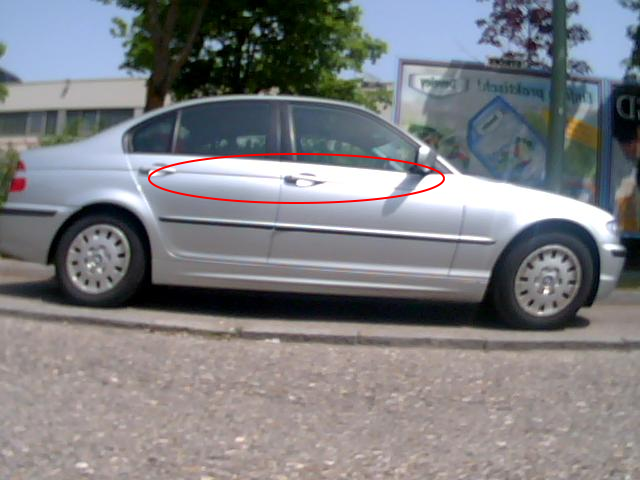
\includegraphics[width=\textwidth, height=0.55\textwidth]{specularity_1_l.png}
		\caption{Αριστερή λήψη}
	\end{subfigure}
	\begin{subfigure}{.49\textwidth}
		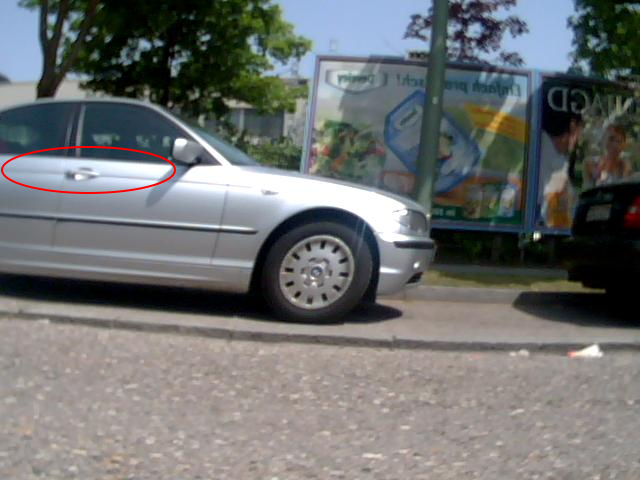
\includegraphics[width=\textwidth, height=0.55\textwidth]{specularity_1_r.png}
		\caption{Δεξιά λήψη}
	\end{subfigure}
	
	\begin{subfigure}{.49\textwidth}
		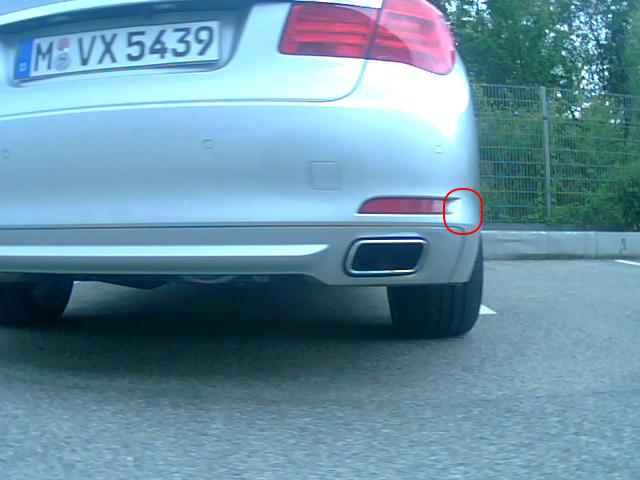
\includegraphics[width=\textwidth, height=0.55\textwidth]{specularity_2_l.png}
		\caption{Αριστερή λήψη}
	\end{subfigure}
	\begin{subfigure}{.49\textwidth}
		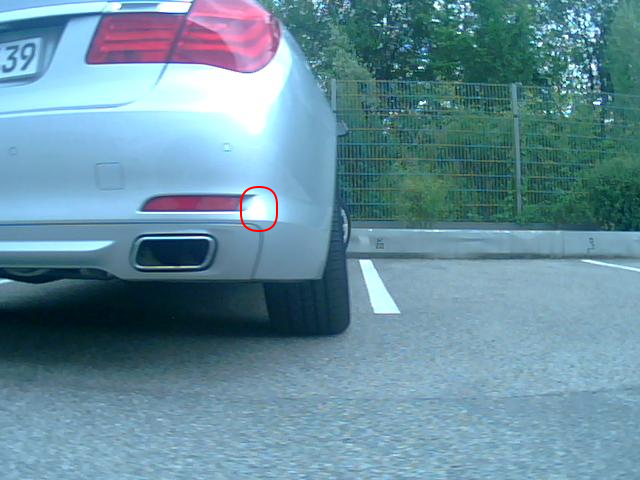
\includegraphics[width=\textwidth, height=0.55\textwidth]{specularity_2_r.png}
		\caption{Δεξιά λήψη}
	\end{subfigure}
	\caption{Φαινόμενο ανάκλασης φωτεινής πηγής. Πηγή: \citep{TUMLesson}}
	\label{fig:specularity}
\end{figure}

\begin{figure}
	\centering
	\begin{subfigure}{.49\textwidth}
		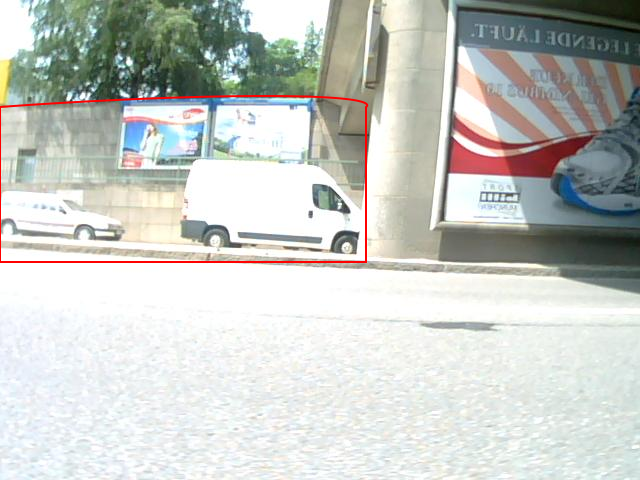
\includegraphics[width=\textwidth, height=0.55\textwidth]{photometric_variation_intense_l.png}
		\caption{Αριστερή λήψη}
	\end{subfigure}
	\begin{subfigure}{.49\textwidth}
		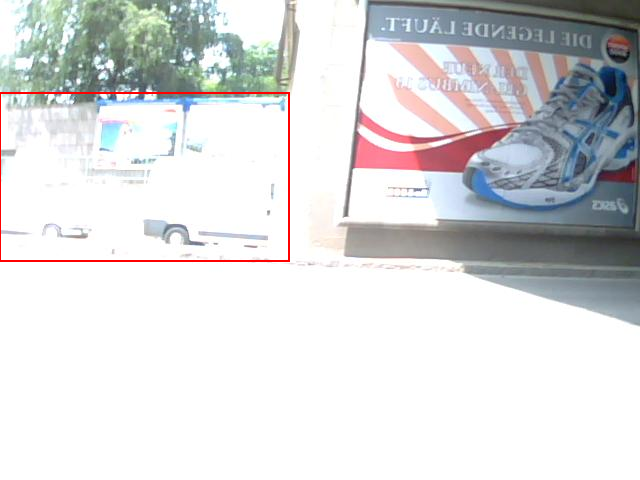
\includegraphics[width=\textwidth, height=0.55\textwidth]{photometric_variation_intense_r.png}
		\caption{Δεξιά λήψη}
	\end{subfigure}

	\begin{subfigure}{.49\textwidth}
		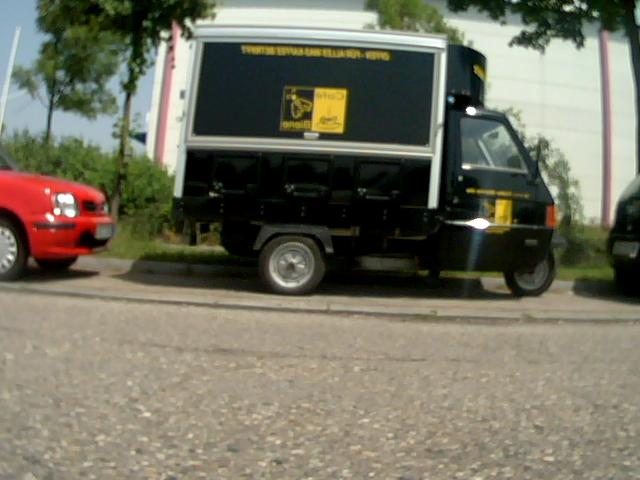
\includegraphics[width=\textwidth, height=0.55\textwidth]{photometric_variation_mild_l.png}
		\caption{Αριστερή λήψη}
	\end{subfigure}
	\begin{subfigure}{.49\textwidth}
		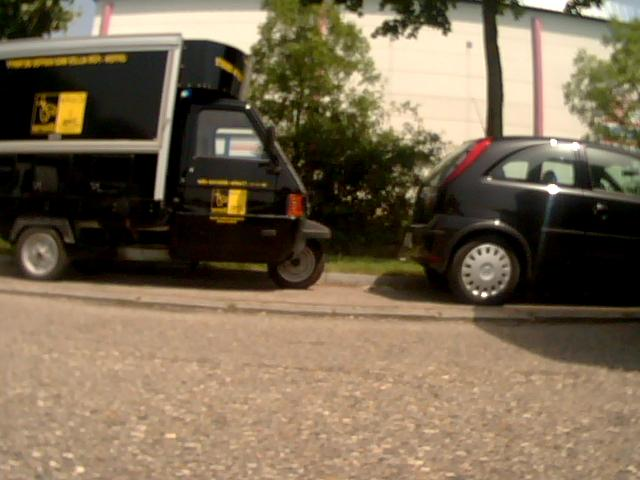
\includegraphics[width=\textwidth, height=0.55\textwidth]{photometric_variation_mild_r.png}
		\caption{Δεξιά λήψη}
	\end{subfigure}
	\caption{Φαινόμενο φωτομετρικής απόκλισης. Πηγή: \citep{TUMLesson}}
	\label{fig:photometric_variation}
\end{figure}

\begin{figure}
	\centering
	\begin{subfigure}{.3\textwidth}
		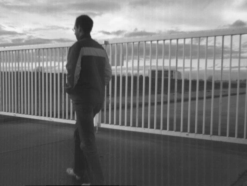
\includegraphics[width=\textwidth, height=0.55\textwidth]{repetitive1.png}
	\end{subfigure}
	\begin{subfigure}{.3\textwidth}
		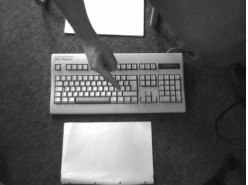
\includegraphics[width=\textwidth, height=0.55\textwidth]{repetitive2.png}
	\end{subfigure}
	\begin{subfigure}{.3\textwidth}
		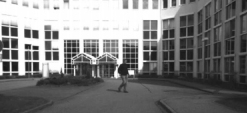
\includegraphics[width=\textwidth, height=0.55\textwidth]{repetitive4.png}
	\end{subfigure}
	\caption{Επαναλαμβανόμενα μοτίβα και υφές}
	\label{fig:repetitive}
\end{figure}

\begin{figure}
	\centering
	\begin{subfigure}{.49\textwidth}
		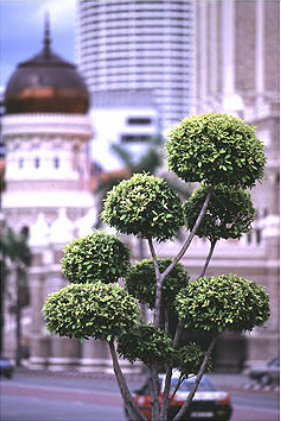
\includegraphics[width=\textwidth]{focus1.png}
		\caption{Αριστερή λήψη}
	\end{subfigure}
	\begin{subfigure}{.49\textwidth}
		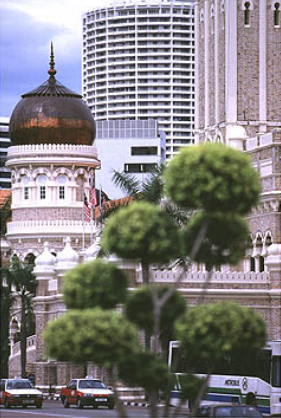
\includegraphics[width=\textwidth]{focus2.png}
		\caption{Δεξιά λήψη}
	\end{subfigure}
	\caption{Διαφορετική εστίαση σε κάθε λήψη}
	\label{fig:different_focus}
\end{figure}

Τα παραπάνω φαινόμενα αμφισβητούν, περισσότερο ή λιγότερο, τοπικά ή ολικά, τις αρχικές υποθέσεις στις οποίες βασίζονται οι μεθοδολογίες επίλυσης του προβλήματος της στερεοσκοπικής αντιστοίχησης απαιτώντας ειδική αντιμετώπιση.

%%%%%%%%%%%%%%%%%%%%%%%%%%%%%%%%%%%%%%%%%%%%%%%%%%%%%%%%%%%%%%%%%%%%%%%%%%%%%%%%%%%%%%%%%%%%%%%%%%%%%%%%%%%%%%%%%%%%%%%%%%%%
%%%%%%%%%%%%%%%%%%%%%%%%%%%%%%%%%%%%%%%%%%%%%%%%%%%%%%%%%%%%%%%%%%%%%%%%%%%%%%%%%%%%%%%%%%%%%%%%%%%%%%%%%%%%%%%%%%%%%%%%%%%%
%%%%%%%%%%%%%%%%%%%%%%%%%%%%%%%%%%%%%%%%%%%%%%%%%%%%%%%%%%%%%%%%%%%%%%%%%%%%%%%%%%%%%%%%%%%%%%%%%%%%%%%%%%%%%%%%%%%%%%%%%%%%

\section{Ανάλυση της στερεοσκοπικής αντιστοίχησης σε επιμέρους υποπροβλήματα}

Οι \e Scharstein et Szeliski \g \citep{in2002taxonomy} επιμερίζουν τους αλγορίθμους επίλυσης προβλημάτων στερεοσκοπικής όρασης σε 4 βήματα:

\begin{enumerate}
	\item Υπολογισμός κόστους αντιστοίχησης \e (matching cost computation) \g
	\item Άθροιση κόστους \e (cost aggregation) \g
	\item Υπολογισμός/βελτιστοποίηση χάρτη παράλλαξης \e (disparity computation/optimization) \g
	\item Διόρθωση χάρτη παράλλαξης \e (disparity refinement) \g
\end{enumerate}

Οι \e Hirschmuller et Scharstein \g \citep{hirschmuller2007evaluation} ομαδοποίησαν περαιτέρω την παραπάνω κατηγοριοποίηση προτείνοντας δύο μόνο βήματα:

\begin{enumerate}
	\item Αρχικοποίηση κόστους αντιστοίχισης \e (matching cost initialization) \g
	\item Στερεοσκοπική μέθοδος \e (Stereo method) \g
\end{enumerate}

Στην εργασία θα ακολουθήσουμε την ταξινόμηση των \e Hirschmuller et Scharstein. \g

%%%%%%%%%%%%%%%%%%%%%%%%%%%%%%%%%%%%%%%%%%%%%%%%%%%%%%%%%%%%%%%%%%%%%%%%%%%%%%%%%%%%%%%%%%%%%%%%%%%%%%%%%%%%%%%%%%%%%%%%%%%%
%%%%%%%%%%%%%%%%%%%%%%%%%%%%%%%%%%%%%%%%%%%%%%%%%%%%%%%%%%%%%%%%%%%%%%%%%%%%%%%%%%%%%%%%%%%%%%%%%%%%%%%%%%%%%%%%%%%%%%%%%%%%
%%%%%%%%%%%%%%%%%%%%%%%%%%%%%%%%%%%%%%%%%%%%%%%%%%%%%%%%%%%%%%%%%%%%%%%%%%%%%%%%%%%%%%%%%%%%%%%%%%%%%%%%%%%%%%%%%%%%%%%%%%%%

\section{Αρχικοποίηση κόστους αντιστοίχισης}

Στον παρών κεφάλαιο, όταν αναφερόμαστε σε σημείο $p=(x,y)$ της εικόνας εννοούμε το αντίστοιχο \e pixel. \g Επομένως, οι τιμές $x,y$ είναι διακριτές με πεδίο τιμών \e $[0,\ldots,width-1]$ \g και \e $[0,\ldots,height-1]$ \g αντίστοιχα. Κατά τον περιορισμό \ref{prop:disparity_limit} ορίζουμε ένα μέγιστο όριο στις υποψήφιες τιμές παράλλαξης που ερευνούμε και το ονομάζουμε $\mathtt{max\_disparity}$. Στόχος του παρόντος βήματος είναι για κάθε θέση $p$ της εικόνας αναφοράς και για πιθανή παράλλαξη $d$ να αναθέσουμε μια τιμή. Η τιμή αυτή θα προέλθει από την σύγκριση της γειτονιάς του $p$ με την αντίστοιχη γειτονιά του κάθε υποψήφιου σημείου $q = (x-d,y)$ στην έτερη λήψη. Αν η τιμή εκφράζει ομοιότητα, όσο μεγαλύτερη τόσο πιο όμοιες οι συγκρινόμενες γειτονιές, ενώ το αντίθετο ισχύει αν εκφράζει κόστος. Στην παρούσα εργασία επιλέγουμε η τιμή να εκφράζει κόστος. Συμβολίζουμε τη γειτονιά ενός σημείου $p$ με το σύμβολο $N_p$, και την ορίζουμε ως ένα τετράγωνο χωρίο με κέντρο το σημείο $p$. Το μέγεθος της γειτονιάς, δηλαδή η πλευρά του τετραγώνου, είναι μια ελεύθερη παράμετρος προς πειραματισμό.

Επομένως κατά το βήμα αυτό δημιουργούμε έναν τρισδιάστατο πίνακα κόστους:

$$ C(d,x,y) : \mathbb{Z}^3 \rightarrow \mathbb{R} : C(d,x,y) = cost(I^L(x,y),I^R(x-d,y))$$

Η συνάρτηση $cost$ είναι μια μετρική ομοιότητας. Παρακάτω παρατίθενται οι πιο γνωστές μετρικές που έχουν εφαρμοστεί:

\begin{itemize}
\item "Άθροισμα απόλυτων διαφορών" (\e sum of absolute differences - SAD):\citep{hannah1974computer}
$$ C(d,p) = -\sum_{q \in N_p} |I^L(q) - I^R(q-d)| $$ \g
Η πιο απλή μέθοδος, η οποία αξιοποιείται ως επίδοση βάσης. Βασίζεται στην παραδοχή ότι η φωτεινότητα μένει σταθερή κατά την προβολή μιας γειτονιάς σημείων του χώρου σε δυο διαφορετικές λήψεις.

\item "Άθροισμα τετραγώνων διαφορών" (\e sum of square differences - SSD):\citep{kanade1997development}
$$ C(d,p) = -\sum_{q \in N_p} { \left( I^L(q) - I^R(q-d) \right) }^2 $$ \g
Βασίζεται στις ίδιες παραδοχές με την μέθοδο \e SAD. \g Λόγω του τετραγώνου εμφανίζει εντονότερη πόλωση στα μεγάλα σφάλματα.

\item "Κανονικοποιημένη ετεροσυσχέτιση" ή "ομοιότητα συνημιτόνου":
\begin{equation*}
C(\mathbf{p}, d) = \frac{\sum_{\mathbf{q} \in \mathcal{N}_{\mathbf{p}}} I^L(\mathbf{q}) I^R(\mathbf{q} - \mathbf{d})}
{\sqrt{\sum_{\mathbf{q} \in \mathcal{N}_{\mathbf{p}}} I^L(\mathbf{q})^2 \sum_{\mathbf{q} \in \mathcal{N}_{\mathbf{p}}} I^R(\mathbf{q} - \mathbf{d})^2 }}.
\end{equation*}

\item Απόσταση \e Hamming \g σε μετασχηματισμό \e Census. \g Αρχικά εφαρμόζουμε στη γειτονιά $\mathcal{N}_{\mathbf{p}}$ τον μετασχηματισμό \e Census. \g Ο μετασχηματισμός αυτός συγκρίνει την φωτεινότητα κάθε σημείου της γειτονιάς $\mathcal{N}_{\mathbf{p}}$ με την φωτεινότητα του κεντρικού \e pixel, \g αποθηκεύοντας την ετικέτα $1$ αν είναι φωτεινότερο το περιφερειακό σημείο και $0$ σε αντίθετη περίπτωση:

\begin{equation*}
	\mathbf{c}_{i,j} = \begin{cases}
		1 & \text{εάν} \: |I(i,j) - I_c| \geqslant 0\\
		0 & \text{εάν} \: |I(i,j) - I_c| < 0
	\end{cases}
\end{equation*}

Έπειτα μετατρέπουμε τον πίνακα $\mathbf{c}_{i,j}$ σε ένα δυαδικό διάνυσμα $census(\mathbf{p})$ $n$ θέσεων, όσο και το μέγεθος της γειτονιάς. Τέλος εφαρμόζουμε την απόσταση \e Hamming \g στα διανύσματα $census$ των συγκρινόμενων περιοχών:

$$XNOR = census(I^L(\mathcal{N}_{\mathbf{p}}) \odot census(I^R(\mathcal{N}_{\mathbf{\mathbf{p} - \mathbf{d}}}) $$
$$C(\mathbf{p}, d) = XNOR\cdot XNOR$$
\end{itemize}

Έχουν προταθεί πολλές ακόμη μέθοδοι αρχικοποίησης του πίνακα κόστους. Το βήμα αυτό είναι το σημαντικότερο στην αλληλουχία βημάτων που καταλήγει στον υπολογισμό του χάρτη παράλλαξης και γι' αυτό η βιβλιογραφία είναι μεγάλη. Στο επόμενο κεφάλαιο θα δούμε πως με τη χρήση μηχανικής μάθησης μέσω τεχνητού νευρωνικού δικτύου, καταφέρνουμε την αρχικοποίηση πίνακα κόστους πολύ μεγαλύτερης ακρίβειας από αυτόν που πετυχαίνουν όλες οι παραπάνω μέθοδοι.

%%%%%%%%%%%%%%%%%%%%%%%%%%%%%%%%%%%%%%%%%%%%%%%%%%%%%%%%%%%%%%%%%%%%%%%%%%%%%%%%%%%%%%%%%%%%%%%%%%%%%%%%%%%%%%%%%%%%%%%%%%%%
%%%%%%%%%%%%%%%%%%%%%%%%%%%%%%%%%%%%%%%%%%%%%%%%%%%%%%%%%%%%%%%%%%%%%%%%%%%%%%%%%%%%%%%%%%%%%%%%%%%%%%%%%%%%%%%%%%%%%%%%%%%%
%%%%%%%%%%%%%%%%%%%%%%%%%%%%%%%%%%%%%%%%%%%%%%%%%%%%%%%%%%%%%%%%%%%%%%%%%%%%%%%%%%%%%%%%%%%%%%%%%%%%%%%%%%%%%%%%%%%%%%%%%%%%

\section{Στερεοσκοπική Μέθοδος \texorpdfstring{\e (stereo method) \g}{TEXT}}

Η αρχικοποίηση του όγκου κόστους $C$ περιέχει αρκετές λανθασμένες εκτιμήσεις, τοποθετημένες στα σημεία που αναιρούνται οι περιορισμοί της στερεοσκοπικής αντιστοίχησης (αποκρύψεις, φωτομετρικές αλλοιώσεις, ομοιόμορφες περιοχές κ.α.). Στην στερεοσκοπική μέθοδο, εφαρμόζουμε τεχνικές που βελτιώνουν τις αρχικές εκτιμήσεις, οδηγώντας σε πιο ακριβή τελικό χάρτη παράλλαξης.

Θα αξιοποιήσουμε κυρίως τις μεθόδους που χρησιμοποίησαν οι \e Mei et al. \g (2011) \cite{mei2011building} κι αναπροσάρμοσαν οι \e Zbontar et LeCun (2016) \g \cite{zbontar2016stereo}.

\subsection{Άθροιση κόστους σε περιοχή υποστήριξης}

Βασιζόμενοι στην υπόθεση "ομοιότητας γειτονιάς" (η οποία καταρρέει τοπικά σε ασυνέχειες βάθους), μπορούμε να αναθέσουμε σε κάθε \e pixel \g τον μέσο όρο των αρχικοποιημένων τιμών κόστους ολόκληρης της γειτονιάς του. Υποθέτουμε δηλαδή ότι αν ένα σημείο $\mathbf{p}$ έχει παράλλαξη $d$ τότε και τα γειτονικά του σημεία θα βρίσκονται σε ίδια ή κοντινή παράλλαξη, αρκεί να μη μεταβαίνουμε από ένα αντικείμενο σε ένα άλλο.

Το σχήμα και το μέγεθος της γειτονιάς, που στο εξής θα ονομάζουμε περιοχή υποστήριξης \e (support region) \g μπορούν να προσδιοριστούν με δύο τρόπους:

\begin{itemize}
	\item Ως μια ορθογώνια περιοχή προαποφασισμένου μεγέθους.
	\item Ως μια προσαρμοσμένη περιοχή, διαφορετική για κάθε σημείο $\mathbf{p}$.
\end{itemize}

\subsubsection{Ορθογώνια περιοχή}
Η περιοχή υποστήριξης είναι ένα τετράγωνο χωρίο το μέγεθος του οποίου επιλέγεται πειραματικά. Η επιλογή: 

\begin{itemize}
	\item μικρής περιοχής υποστήριξης προκαλεί ασάφειες (πολλές διαφορετικές τιμές παράλλαξης με παρόμοιο κόστος), καθώς δεν συνδυάζει αρκετή πληροφορία. Έτσι προκαλείται ένας χάρτης παράλλαξης αρκετά "τραχύς" με πολλές εξωκείμενες τιμές. \ref{fig:small_window}
	\item μεγάλης περιοχής υποστήριξης έχει τα αντίστροφα αποτελέσματα. Συνδυάζει αρκετή πληροφορία, δημιουργώντας λείο χάρτη παράλλαξης, αλλά αδυνατεί να εντοπίσει τις ακμές τις οποίες και θολώνει καθώς πάσχει σε περιοχές ασυνέχειας βάθους, όπου οι αποκρύψεις καταστρατηγούν την "ομοιότητα γειτονιάς". \ref{fig:large_window}
\end{itemize}

Η μαθηματική πράξη που υλοποιεί την παραπάνω διεργασία είναι η χωρική συνέλιξη με χωρικό φίλτρο μέσου όρου:

\begin{align*}
	\mathtt{for} \: \: & \mathtt{d = 0:max\_disparity} \\
	& C_{agg}(d,:,:) = C_{init}(d,:,:) \ast h
\end{align*}



όπου $C_{init}$ ο αρχικός πίνακας κόστους, $C_{agg}$ αυτός που προκύπτει μετά την συνέλιξη και $h$ το φίλτρο μέσου όρου.

Η παραπάνω πράξη μπορεί μάλιστα να εφαρμοστεί κατ' επανάληψη, που ισοδυναμεί βαθμιαία με συνέλιξη με γκαουσιανό φίλτρο μεγαλύτερων διαστάσεων, όπως αποδεικνύεται στο παράρτημα \ref{appendix:mean2gaussian}.

\begin{figure}
	\centering
	\begin{subfigure}{.33\textwidth}
		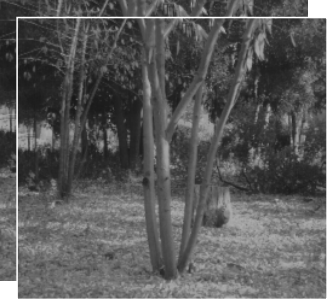
\includegraphics[width=\textwidth]{cost_aggregation1.png}
		\caption{στερεοσκοπικό ζεύγος}
	\end{subfigure}
	\begin{subfigure}{.33\textwidth}
		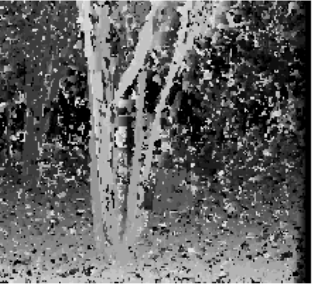
\includegraphics[width=\textwidth]{cost_aggregation2.png}
		\caption{μικρό παράθυρο $w=3$ pixels}
		\label{fig:small_window}
	\end{subfigure}
		\begin{subfigure}{.33\textwidth}
		\includegraphics[width=\textwidth]{cost_aggregation3.png}
		\caption{μεγάλο παράθυρο $w=20$ pixels}
		\label{fig:large_window}
	\end{subfigure}
	\caption{χάρτης παράλλαξης για μεταβλητό μέγεθος παραθύρου}
\end{figure}


\subsubsection{Προσαρμοσμένη περιοχή υποστήριξης}

Ο ορισμός ενιαίας περιοχής υποστήριξης για όλα τα σημεία προκαλεί τα παραπάνω προβλήματα. Επιθυμούμε την δημιουργία περιοχής υποστήριξης διαφορετικού μεγέθους και σχήματος ανά σημείο. Στόχος είναι η περιοχή υποστήριξης να μην περιλαμβάνει μεταβάσεις από ένα αντικείμενο σε ένα άλλο. Έτσι οι μέσοι όροι θα συνδυάζουν πληροφορία από γειτονικά \e pixels \g που ανήκουν στο ίδιο αντικείμενο και άρα έχουν ίδια ή παρόμοια τιμή παράλλαξης. 

Βασιζόμαστε στην υπόθεση ότι η μετάβαση από ένα αντικείμενο σε ένα άλλο αποτυπώνεται στο πέτασμα μέσω απότομης αλλαγής στη φωτεινότητα των \e pixels. \g \citep{lu2008anisotropic} Ακολουθώντας την μεθοδολογία που πρότειναν οι \e Zhang et al. (2009) \g \cite{zhang2009cross}, αντιστοιχίζουμε σε κάθε \e pixel \g τέσσερις τιμές που συγκροτούν έναν σταυρό. Συγκεκριμένα, οι τέσσερις τιμές $[v_{p}^-, v_{p}^+, h_{p}^-, h_{p}^+]$ δηλώνουν πόσο εκτείνεται ο σταυρός στις τέσσερις κατευθύνσεις: πάνω, κάτω - κάθετος άξονας - και αριστερά, δεξιά - οριζόντιος άξονας.

Αποφασίζουμε την τιμή των $[v_{p}^-, v_{p}^+, h_{p}^-, h_{p}^+]$ που αντιστοιχούν στο \e pixel \g $p$ ακολουθώντας δύο κριτήρια. Μετατοπιζόμαστε κατά μήκος της κάθε κατεύθυνσης όσο τηρούνται οι περιορισμοί: 

\begin{itemize}
	\item \e $|I(\mathbf{p}) - I(\mathbf{p'})| < \texttt{intensity\_threshold}$: \g η διαφορά στη φωτεινότητα μεταξύ του υπό εξέταση \e pixel \g $\mathbf{p}$ και του $\mathbf{p'}$ είναι μικρότερο ενός ορίου που θέτουμε ως παράμετρο. Όσο μικρότερη τιμή ορίου, τόσο αυξανόμενη ευαισθησία στην ανεύρεση συνόρου.			
	\item \e $\|\mathbf{p} - \mathbf{p'}\| < \texttt{distance\_threshold}$: \g η μέγιστη τιμή προς κάθε κατεύθυνση περιορίζεται από το όριο  \e $\texttt{distance\_threshold}$ \g επιβάλλοντας περιορισμό στο μέγιστο εμβαδό της περιοχής υποστήριξης.
\end{itemize}

Αφού υπολογιστούν οι τέσσερις τιμές \e $[v_{p}^-, v_{p}^+, h_{p}^-, h_{p}^+]  \forall \mathbf{p}$\g, η περιοχή υποστήριξης του \e$\mathbf{p}$ \g υπολογίζεται ως η ένωση των τιμών $[h_{p}^-, h_{p}^+]$ όλων των θέσεων \e$\mathbf{q}$ \g κατά μήκος του κάθετου άξονα του \e $\mathbf{p}$ \g, όπως φαίνεται στο σχήμα \ref{fig:cbca_cross}

Η τελική επιλογή περιοχής υποστήριξης πρέπει λαμβάνει υπ' όψη και την αντίστοιχη περιοχή στο αντίστοιχο \e pixel \g της έτερης λήψης. Επομένως, συμβολίζοντας \e $U^{L}(\mathbf{p})$ \g την περιοχή υποστήριξης στην αριστερή λήψη, \e $U^{R}(\mathbf{p})$ \g στην δεξιά, η τελική περιοχή υποστήριξης για την υπό εξέταση παράλλαξη $d$ είναι η: \e

\begin{gather*}
U_d(\mathbf{p}) = U^{L}(\mathbf{p}) \cup  U^{R}(\mathbf{p-d}) \Rightarrow\\
U_d(\mathbf{p}) = \{\mathbf{q} | \mathbf{q} \in U^L(\mathbf{p}), \mathbf{q}-\mathbf{d}
\in U^R(\mathbf{p}-\mathbf{d})\}
\end{gather*}\g

Στο σχήμα \ref{fig:cbca_tsukuba}, φαίνεται ότι η προσαρμοσμένη περιοχή υποστήριξης αποδίδει με ικανοποιητική ακρίβεια, καταφέρνοντας να περιορίσει τις περιοχές υποστήριξης εντός των ίδιων αντικειμένων και αποφεύγοντας την εμπλοκή εξωκείμενων τιμών στον υπολογισμό των μέσων όρων. 

Η υπολογιστική πολυπλοκότητα του υπολογισμού της γειτονιάς για κάθε σημείο είναι \e $O(H \cdot W \cdot \texttt{distance\_threshold})$, \g ενώ για την άθροιση του κόστους $O(H \cdot W \cdot D \cdot (2 \cdot \texttt{distance\_threshold})^2)$ 

\begin{figure}
	\centering
	\includegraphics[width=0.5\textwidth]{cbca_cross.png}
	\caption{παράδειγμα δημιουργίας περιοχής υποστήριξης τυχαίου \e pixel $\mathbf{p}$ \g. Αφού, υπολογιστούν οι τιμές $[v_{p}^-, v_{p}^+, h_{p}^-, h_{p}^+]$ υπολογίζονται οι οριζόντιοι άξονες όλων των θέσεων \e $\mathbf{q}$ \g κατά μήκος του κάθετου άξονα}
	\label{fig:cbca_cross}
\end{figure}

\begin{figure}
	\centering
	\includegraphics[width=1\textwidth]{cbca_tsukuba.png}
	\caption{εφαρμογή μεθόδου υπολογισμού προσαρμόσιμων περιοχών υποστήριξης.}
	\label{fig:cbca_tsukuba}
\end{figure}

\subsection{Ημικαθολική αντιστοίχηση \texorpdfstring{\e (semi-global matching) \g}{TEXT}}

Η μέθοδος άθροισης κόστους σε περιοχές υποστήριξης του προηγούμενο κεφαλαίου πετυχαίνει την τοπική εξομάλυνση των τιμών του κόστους. Οι νέες τιμές κόστους που υπολογίζει για κάθε \e pixel \g εξαρτώνται μόνο από τις τιμές της "γειτονιάς" του.

Η ημικαθολική αντιστοίχηση επιχειρεί να επιβάλει εξωτερικούς περιορισμούς που λαμβάνουν υπ' όψιν τις τιμές κόστους όλης της εικόνας καθολικά κι όχι ξεχωριστά κάθε γειτονιάς, όπως η προηγούμενη μέθοδος. Έτσι, επιδιώκει τον σχηματισμό ενός καθολικά ομαλού χάρτη παράλλαξης κι όχι ομαλού κατά γειτονιές μόνο. Όπως είναι λογικό, η πρόκληση που αντιμετωπίζει αφορά τις ασυνέχειες βάθους, τις οποίες πρέπει να εντοπίσει και να χειριστεί κατάλληλα, ώστε να μην προκύψει χάρτης παράλλαξης με θολωμένες \e (blur)\g τις άκρες των αντικειμένων.

Ορίζουμε μια συνάρτηση αναφοράς (συνήθως αποκαλείται μεταφορικά συνάρτηση ενέργειας, χωρίς να σχετίζεται άμεσα με την φυσική έννοια της ενέργειας) $E$ που εξαρτάται από τον χάρτη παράλλαξης $D$ και τον αρχικοποιημένο πίνακα κόστους $C$. Στο παρών βήμα θεωρούμε σταθερό τον πίνακα κόστους $C$ και μεταβλητό τον χάρτη παράλλαξης $D$, επομένως συμβολίζουμε την συνάρτησή μας ως $E_C(D)$ και την ορίζουμε ως:

\begin{multline}
\label{eq:energy_function}
E_C(D) = \sum_{\mathbf{p}} \biggl( C(\mathbf{p}, D(\mathbf{p}))
+ \sum_{\mathbf{q} \in \mathcal{N}_{\mathbf{p}}} P_1 \cdot 1\{|D(\mathbf{p}) - D(\mathbf{q})| = 1\} \\
+ \sum_{\mathbf{q} \in \mathcal{N}_{\mathbf{p}}} P_2 \cdot 1\{|D(\mathbf{p}) - D(\mathbf{q})| > 1\} \biggr), 
\end{multline}

Η συνάρτηση $1\{\cdot\}$ ισούται με \e
  
\[
1 \{ \text{statement} \} =
 	\left\{\begin{array}{lr}
	1 , & \text{if, statement: True} \\ 
	0 , & \text{if, statement: False}
\end{array}\right\}
\]

\g 

Στην συνάρτηση \ref{eq:energy_function} ο όρος:

\begin{itemize}
	\item $\sum_{\mathbf{p}} C(\mathbf{p}, D(\mathbf{p}))$ "τιμωρεί" τις επιλογές παράλλαξης υψηλού κόστους
	\item $\sum_{\mathbf{q} \in \mathcal{N}_{\mathbf{p}}} P_1 \cdot 1\{|D(\mathbf{p}) - D(\mathbf{q})| = 1\}$ "τιμωρεί" με την τιμή $P_1$ κάθε γειτονικό \e pixel \g με παράλλαξη που διαφέρει κατά 1
	\item $\sum_{\mathbf{q} \in \mathcal{N}_{\mathbf{p}}} P_2 \cdot 1\{|D(\mathbf{p}) - D(\mathbf{q})| > 1\}$ "τιμωρεί" με την τιμή $P_2>P_1$ κάθε γειτονικό \e pixel \g με παράλλαξη που διαφέρει περισσότερο από 1
\end{itemize}

Η τιμές $P_1, P_2$ δεν πρέπει να παραμείνουν αμετάβλητες σε όλο το εύρος της εικόνας. Μια τέτοια προσέγγιση θα "τιμωρούσε" την απότομη μεταβολή στην παράλλαξη γειτονικών \e pixel \g που βρίσκονται σε διαφορετικό επίπεδο, μη επιτρέποντας την ασυνέχεια σε ασυνεχείς επιφάνειες. Αντιθέτως, επιθυμούμε μεροληπτική συμπεριφορά που θα ευνοεί τις ασυνέχειες σε ασυνεχείς επιφάνειες και θα τις τιμωρεί σε συνεχείς, σεβόμενοι την αντίστοιχη υπόθεση. Θα αξιοποιήσουμε την μέθοδο της ανίχνευσης ακμών από τις απότομες μεταβάσεις στη φωτεινότητα. Ορίζουμε: \e
\[
	\begin{array}{c}
		diff_l = |I^L(\mathbf{p}) - I^L(\mathbf{q})|\quad, \quad \mathbf{p} \in I^L, \quad \mathbf{q} \in \mathcal{N}_{\mathbf{p}} \\
	 \\
		diff_r = |I^R(\mathbf{p}-\mathbf{d}) - I^R(\mathbf{q}-\mathbf{d})|\quad , \quad d: \texttt{disparity of p}
	\end{array}
\]

\g κι επιλέγουμε την τιμή των $P_1, P_2$ σύμφωνα με τους κανόνες: \e

\[ \begin{array}{lll} 
P_1 = \texttt{P1\_ref}, &P_2 = \texttt{P2\_ref} & 
\text{if $diff_l < \texttt{thres}, diff_r < \texttt{thres}$} \\ 
P_1 = \texttt{P1\_ref} / \texttt{big\_factor}, &P_2 = \texttt{P2\_ref} / \texttt{big\_factor} & 
\text{if $diff_l \geq \texttt{thres}, diff_r \geq \texttt{thres}$} \\ 
P_1 = \texttt{P1\_ref} / \texttt{small\_factor}, &P_2 = \texttt{P2\_ref} / \texttt{small\_factor} & 
\text{otherwise.} \\ 
\end{array} \]

\g Οι υπερπαράμετροι της μεθοδολογίας είναι οι

\begin{itemize}
	\item \e $\texttt{P1\_ref, P2\_ref}$ \g που εκφράζουν την βασική τιμή αναφοράς για τις ασυνέχειες στην τιμή της παράλλαξης
	\item \e $\texttt{thres}$ \g, όριο στην διαφορά της φωτεινότητας
	\item \e $\texttt{small\_factor}$ \g, διαιρεί την τιμή αναφοράς όταν μία εκ των τιμών $diff_l$, $diff_r$ ξεπεράσει το όριο διαφοράς φωτεινότητας
	\item \e $\texttt{big\_factor}$ \g, διαιρεί την τιμή αναφοράς όταν οι $diff_l$, $diff_r$ αμφότερες ξεπεράσουν το όριο διαφοράς φωτεινότητας
\end{itemize}

\subsubsection{Επίλυση του προβλήματος ημικαθολικής αντιστοίχησης}

Το πρόβλημα ελαχιστοποίησης της συνάρτησης $E_C(D)$ εμφανίζει δυσκολία επίλυσης για δύο λόγους:
\begin{itemize}
	\item Η συνάρτηση $E_C(D)$ δεν είναι συνεχής ώστε να προσεγγίσουμε το ελάχιστό της μέσω μεθοδολογιών πρώτης παραγώγου 
	\item Οι πιθανές τιμές $D$ είναι \e $(m \times n)^{\text{max\_disparity}}$ \g που δημιουργεί μη αντιμετωπίσιμη υπολογιστική πολυπλοκότητα. Για παράδειγμα, μια εικόνα πολύ μικρής ανάλυσης \e $50\times100 \text{pixels}$ \g με μέγιστη παράλλαξη μόλις τα \e $10 \text{pixels}$ \g δημιουργεί χώρο $(50 \times 100)^{10} \approx 10^{37}$ πιθανών τιμών.
\end{itemize}

\g
Είναι υπολογιστικά αδύνατη η επίλυση του προβλήματος προς όλες τις κατευθύνσεις ταυτόχρονα. Αναγκαστικά, συμβιβαζόμαστε στην επίλυσή του προς μία κατεύθυνση $\mathbf{r}$ τη φορά με τη βοήθεια δυναμικού προγραμματισμού. Φυσικά, αυτός ο συμβιβασμός μας εγγυάται την επιβολή των εξωτερικών περιορισμών ομαλότητας \textbf{μόνο} στις κατευθύνσεις που θα τον εφαρμόσουμε. 

Ο \e Hirschmüller (2008) \g \citep{hirschmuller2008stereo} πρότεινε την ελαχιστοποίηση της ενέργειας σε 16 κατευθύνσεις, όπως φαίνονται στην εικόνα \ref{fig:sgm1}, και τον τελικό υπολογισμό του μέσου όρου αυτών.

\subsubsection{Επίλυση του προβλήματος ημικαθολικής αντιστοίχησης σε μία κατεύθυνση}

Η επίλυση του προβλήματος σε μια προαποφασισμένη κατεύθυνση μπορεί να υλοποιηθεί με χρήση δυναμικού προγραμματισμού. Οι νέες τιμές του πίνακα κόστους $C_{\mathbf{r}}(\mathbf{p}, d)$ υπολογίζονται σύμφωνα με την αναδρομική σχέση:

\begin{multline*} \label{sgm_recursive} C_{\mathbf{r}}(\mathbf{p}, d) = C(\mathbf{p},
d) - \min_k C_r(\mathbf{p} - \mathbf{r}, k) + \min\biggl\{ C_r(\mathbf{p} -
\mathbf{r}, d), C_r(\mathbf{p} - \mathbf{r}, d - 1) + P_1,\\ C_r(\mathbf{p} -
\mathbf{r}, d + 1) + P_1, \min_k C_{\mathbf{r}}(\mathbf{p} - \mathbf{r}, k) +
P_2 \biggr\}  \end{multline*}

Με αυτήν την μέθοδο η υπολογιστική πολυπλοκότητα του αλγορίθμου είναι $O(D\cdot H \cdot W)$ ανά κατεύθυνση.

\begin{figure}
	\centering
	\includegraphics[width=1\textwidth]{sgm1.png}
	\caption{οι 16 κατευθύνσεις που προτάθηκαν από τον \e Hirschmüller (2008) \g \citep{hirschmuller2008stereo}}
	\label{fig:sgm1}
\end{figure}

\begin{figure}
	\centering
	\begin{subfigure}{\textwidth}
		\includegraphics[width=\textwidth]{sgm_tsukuba.jpg}
		\caption{Στερεοσκοπικό ζεύγος από το αρχείο \e Middlebury \citep{scharstein2014high} \g}
		\label{fig:sgm_tsukuba}
	\end{subfigure}
	
	\begin{subfigure}{\textwidth}
		\includegraphics[width=\textwidth, height = 8cm]{sgm_tsukuba_1.jpg}
		\caption{Εφαρμογή του αλγορίθμου ημικαθολικής αντιστοίχησης μόνο κατά την οριζόντια κατεύθυνση $\textbf{r} = (1,0)$. Παρατηρούμε ότι η ανυπαρξία κάποιου περιορισμού ομαλότητας προς οποιαδήποτε άλλη κατεύθυνση δημιουργεί τα επονομαζόμενα φαινόμενα ραβδώσεων \e (streaking effects). \g Πηγή: \citep{SGMTutorial}}
		\label{fig:sgm_tsukuba_1}
	\end{subfigure}
\end{figure}

\begin{figure}	
	\begin{subfigure}{\textwidth}
		\includegraphics[width=\textwidth, height = 6.5cm]{sgm_tsukuba_2.jpg}
		\caption{Εφαρμογή του αλγορίθμου στις 8 βασικές κατευθύνσεις: 4 διευθύνσεις (οριζόντια, κάθετη, πρώτη και δεύτερη διαγώνιος) και 2 φορές ανά διεύθυνση. Το φαινόμενο ραβδώσεων εμφανίζεται πάντα σε διαφορετική κατεύθυνση.}
		\label{fig:sgm_tsukuba_2}
	\end{subfigure}
	
	\begin{subfigure}{\textwidth}
		\includegraphics[width=\textwidth, height = 6.5cm]{sgm_tsukuba_3.jpg}
		\caption{Χάρτης παράλλαξης βασισμένος στον μέσο όρο των τιμών που προκύπτουν από τις 8 βασικές κατευθύνσεις. Παρατηρούμε σαφή μείωση του φαινομένου των ραβδώσεων.}
		\label{fig:sgm_tsukuba_3}
	\end{subfigure}
	
	\begin{subfigure}{\textwidth}
		\includegraphics[width=\textwidth]{sgm_tsukuba_4.jpg}
		\caption{αριστερά: Χάρτης παράλλαξης βασισμένος στον μέσο όρο των τιμών που προκύπτουν από τις 16 βασικές κατευθύνσεις, όπως ακριβώς προτάθηκε από τον \e Hirschmüller (2008) \g \citep{hirschmuller2008stereo}. Δεξιά: οι πραγματικές τιμές του χάρτη παράλλαξης μετρημένες εργαστηριακά. Παρατηρούμε την έντονη ομοιότητα στο μεταξύ των δύο εικόνων.}
		\label{fig:sgm_tsukuba_4}
	\end{subfigure}
	
	\caption{Παραδείγματα επίλυσης του προβλήματος της ημικαθολικής αντιστοίχησης σε συγκεκριμένες κατευθύνσεις.  Πηγή: \citep{SGMTutorial} }
	\label{fig:mean_filter_iterations}
\end{figure}

\subsection{Υπολογισμός χάρτη παράλλαξης \texorpdfstring{\e (disparity map computation) \g}{TEXT}}

Μετά την επιβολή των παραπάνω περιορισμών ομαλότητας, ο χάρτης παράλλαξης υπολογίζεται σε κάθε θέση \e $\textbf{p}$ \g ως η παράλλαξη με το ελάχιστο κόστος αντιστοίχησης \e (winner takes it all strategy):

\begin{equation*}
D(\mathbf{p}) = \arg\!\min_d C(\mathbf{p}, d).
\end{equation*}

\g

\subsection{Εντοπισμός εξωκείμενων τιμών στον χάρτη παράλλαξης \texorpdfstring{\e (outlier values detection in disparity map) \g}{TEXT}}

Θεωρούμε δεδομένη μια πρώτη εκτίμηση του χάρτη παράλλαξης $D_{init}$, όπως προέκυψε από το προηγούμενο βήμα. Μας ενδιαφέρει να ερευνήσουμε αν τηρούνται οι περιορισμοί που διατυπώθηκαν στο κεφάλαιο \ref{sec:stereo_constraints}.

Σύμφωνα με τον περιορισμό μοναδικότητας \ref{prop:uniqueness_contraint}, υπάρχει μια "1-1" αντιστρεπτή σχέση που συνδέει τα σημεία των προβαλλόμενων  ειδώλων μιας περιοχής ορατής και από τις δύο λήψεις. Ο περιορισμός αναιρείται σε περίπτωση αποκρύψεων \ref{prop:occlusions}.

Συμβολίζουμε ως $D^L$ τον χάρτη παράλλαξης που προκύπτει θεωρώντας την αριστερή εικόνα $I^L$ ως εικόνα αναφοράς και $D^R$ τον αντίστοιχο με αναφορά στην εικόνα $I^R$. Μελετάμε αν υπάρχει συμφωνία στις τιμές παράλλαξης που προβλέπουν καταλήγοντας σε τρία πιθανά ενδεχόμενα για κάθε $\textbf{p}$:

\begin{itemize}
	\item \textbf{ορθή παράλλαξη}, αν 
		\e $$|D^L(\textbf{p}) - D^R(\textbf{p}-\textbf{d})| \leqslant 1$$ \g διότι οι προβλέψεις ταυτίζονται.
	\item \textbf{απόκρυψη}, αν 
		\e $$|d - D^R(\textbf{p}-\textbf{d})| > 1 \quad \forall d:\lbrace \textbf{p}-\textbf{d} \geqslant 0 \rbrace$$ \g Διατρέχουμε την οριζόντια επιπολική ευθεία στην δεξιά εικόνα κι ελέγχουμε ότι κανένα άλλο \e pixel $\textbf{p'}$ \g δεν αντιστοιχίζεται με το \e pixel $\textbf{p}$ \g. Τότε υποθέτουμε ότι υπάρχει φαινόμενο απόκρυψης. \ref{fig:interpol_occl}
	\item \textbf{αναντιστοιχία για οποιονδήποτε άλλο λόγο}, αν 
		\e $$\exists \quad d:\lbrace \textbf{p}-\textbf{d} \geqslant 0\rbrace \quad \text{\g τέτοιο ώστε\e}:\quad|d - D^R(\textbf{p}-\textbf{d})| \leqslant 1 $$ \g Αν αντίθετα με την προηγούμενη περίπτωση υπάρχει \e pixel $\textbf{p'}$ \g που αντιστοιχίζεται με το \e pixel $\textbf{p}$ \g θεωρούμε ότι για οποιονδήποτε από τους λόγους του κεφαλαίου \ref{sec:stereo_constraints_violation}, έχει παραβιαστεί η ομοιότητα γειτονιάς και έχουμε αστοχία πρόβλεψης.
\end{itemize}

\subsubsection{Διόρθωση τιμών παράλλαξης σε \texorpdfstring{\e pixels \g}{TEXT} με σήμανση "απόκρυψη"}
Για τα \e pixels \g με σήμανση "απόκρυψη", θέλουμε η παράλλαξή τους να υπολογιστεί με βάση γειτονικά \e pixels \g ταυτοποιημένα ως "ορθή παράλλαξη".

Οι \e Mei et. al (2009) \g \citep{mei2011building} προτείνουν τη μέθοδο \e iterative region voting \g (επαναληπτική ψηφοφορία περιοχής υποστήριξης). Σ' αυτήν την μέθοδο δημιουργείται ένα ιστόγραμμα $H_p$ με \e $ d_{max} + 1 $ \g στάθμες, από τις τιμές παράλλαξης των \e pixels \g στην περιοχή υποστήριξης του \e $\textbf{p}$ \g που έχουν σημανθεί ως "ορθή παράλλαξη". Συμβολίζουμε με $d_p^{\ast}$ την υψηλότερη στάθμη. Αν ο αριθμός των ψηφισάντων $S_p$ \e (pixels \g με σήμανση "ορθή παράλλαξη") υπερβαίνει ένα κατώφλι $\tau_S$ και η αναλογία $\dfrac{H_p(d_p^{\ast})}{S_p}$ είναι μεγαλύτερη ενός άλλου ορίου $\tau_H$, τότε η εκτίμηση $d_p^{\ast}$ θεωρείται ασφαλής και ανατίθεται στο \e pixel $\textbf{p}$: \g 

$$ S_p > \tau_s, \quad \dfrac{H_p(d_p^{\ast})}{S_p}>\tau_H$$

Η παραπάνω μέθοδος μπορεί να χρησιμοποιηθεί επαναληπτικά.

Οι \e Zbontar et LeCun (2016) \g \citep{zbontar2016stereo} πρότειναν μια πολύ πιο απλοποιημένη μέθοδο κατά την οποία αναζητούμε το πιο κοντινό \e pixel \g με σήμανση "ορθή παράλλαξη" κατά μήκος της επιπολικής ευθείας κι αναθέτουμε την τιμή της παράλλαξής του στο "κρυμμένο" \e pixel. \g

Η μέθοδος \e Zbontar et LeCun \g είναι πιο συνεπής απέναντι στην στερεοσκοπική γεωμετρία και κυρίως στον περιορισμό μοναδικότητας \ref{prop:uniqueness_contraint}, ενώ η μέθοδος \e Mei et. al \g εμφανίζει μεγαλύτερη ευστάθεια αξιοποιώντας πληροφορία πολλαπλών \e pixels. \g

\subsubsection{Διόρθωση τιμών παράλλαξης σε \texorpdfstring{\e pixels \g}{TEXT} με σήμανση "αναντιστοιχία"}

Τα \e pixels \g με σήμανση "αναντιστοιχία" περιέχουν άστοχη τιμή παράλλαξης. Η αστοχία μπορεί να έχει προέλθει από οποιαδήποτε παραβίαση των περιορισμών την στερεοσκοπικής αντιστοίχησης, όπως παρουσιάστηκαν στο κεφάλαιο \ref{sec:stereo_constraints}, εκτός του περιορισμού μοναδικότητας που προκαλείται από το φαινόμενο αποκρύψεων. Σε κάθε περίπτωση εφόσον εξαιρούμε το ενδεχόμενο απόκρυψης, ισχύουν οι περιορισμοί συνέχειας/ασυνέχειας \ref{prop:disparity_continuity_constraint} και διάταξης παραλλάξεων \ref{prop:ordering_contraint}. Βασιζόμενοι σε αυτές επιθυμούμε την πρόβλεψη της τιμής της παράλλαξης από τα γειτονικά \e pixels. \g

Υλοποιούμε την εξής μεθοδολογία. Κινούμενοι αποκλειστικά εντός της περιοχής υποστήριξης \e $U_d(\textbf{p})$ \g (ώστε να εξασφαλίζουμε πλοήγηση εντός του ίδιου αντικειμένου), εκμεταλλευόμαστε την πληροφορία όλων των \e "pixels" \g με σήμανση "ορθή παράλλαξη". Συμβολίζουμε \e $d_{U_d}(\textbf{p})$ \g το σύνολο των τιμών παράλλαξης των \e pixels, \g εντός της περιοχής υποστήριξης. Ως παράλλαξη του \e pixel $\textbf{p}$ \g αναθέτουμε την διάμεσο του συνόλου \e $d_{U_d}(\textbf{p})$. \g

\begin{figure}
	\centering
	\begin{subfigure}{0.49\textwidth}
		\includegraphics[width=\textwidth]{interpolation_occlusion_l.png}
		\caption{εικόνα 1: χάρτης παράλλαξης $D^L$}
	\end{subfigure}
	\begin{subfigure}{0.49\textwidth}
		\includegraphics[width=\textwidth]{interpolation_occlusion_r.png}
		\caption{εικόνα 2: χάρτης παράλλαξης $D^R$} 
	\end{subfigure}
	\caption{Παράδειγμα αναντιστοιχίας στους χάρτες παράλλαξης $D^L, D^R$ εστιασμένη σε περιοχές απόκρυψης που προκαλούνται λόγω μετάβασης από ένα αντικείμενο σε ένα άλλο}
	\label{fig:interpol_occl}
\end{figure}

\subsection{Βελτιστοποίηση με ακρίβεια υποπίξελ}

Έως τώρα ο χάρτης παράλλαξης περιέχει ακέραιες τιμές. Η παράλλαξη είναι από τη φύση της πραγματικός αριθμός. Προκειμένου να μετατρέψουμε τις ακέραιες τιμές σε πραγματικές, τοποθετούμε μια τετραγωνική καμπύλη \e (quadratic curve) \g ανάμεσα στα γειτονικά κόστη ώστε να υπολογίσουμε έναν νέο χάρτη παράλλαξης:
\e
\begin{equation*}
D_{\text{SE}}(\mathbf{p}) = D_{\text{INT}}(\mathbf{p}) - \frac {C(\mathbf{p}, d + 1) - C(\mathbf{p}, d - 1)} {2 (C(\mathbf{p}, d + 1) - 2 C(\mathbf{p}, d    ) + C(\mathbf{p}, d - 1))},
\end{equation*}
\g

%%%%%%%%%%%%%%%%%%%%%%%%%%%%%%%%%%%%%%%%%%%%%%%%%%%%%%%%%%%%%%%%%%%%%%%%%%%%%%%%%%%%%%%%%%%%%%%%%%%%%%%%%%%%%%%%%%%%%%%%%%%%
%%%%%%%%%%%%%%%%%%%%%%%%%%%%%%%%%%%%%%%%%%%%%%%%%%%%%%%%%%%%%%%%%%%%%%%%%%%%%%%%%%%%%%%%%%%%%%%%%%%%%%%%%%%%%%%%%%%%%%%%%%%%
%%%%%%%%%%%%%%%%%%%%%%%%%%%%%%%%%%%%%%%%%%%%%%%%%%%%%%%%%%%%%%%%%%%%%%%%%%%%%%%%%%%%%%%%%%%%%%%%%%%%%%%%%%%%%%%%%%%%%%%%%%%%

\section{Αξιολόγηση χάρτη παράλλαξης \texorpdfstring{\e (Disparity map evaluation) \g}{TEXT}}

Ο χάρτης παράλλαξης οπτικοποιείται μέσω εικόνας όπου ο χρωματισμός κάθε σημείου ορίζεται από την αντίστοιχη τιμή της παράλλαξης, όπως φαίνεται στην εικόνα \ref{fig:motorcycle_disp_map}. Υπάρχουν δύο βασικές μετρικές αξιολόγησης της ακρίβειας του υπολογισμένου χάρτη παράλλαξης, το "απόλυτο σφάλμα πρόβλεψης" και το "απόλυτο σφάλμα πρόβλεψης με ανώφλι".

\begin{figure}
	\centering
	\begin{subfigure}{0.48\textwidth}
		\includegraphics[width=\textwidth]{motorcycle_l.png}
		\caption{$\textbf{I}^L$}
		\label{fig:motorcycle}
	\end{subfigure}
	\begin{subfigure}{0.48\textwidth}
		\includegraphics[width=\textwidth]{motorcycle_r.png}
		\caption{$\textbf{I}^R$}
	\end{subfigure}
	
	\begin{subfigure}{0.48\textwidth}
		\includegraphics[width=\textwidth]{motorcycle_disp_map_visualization.png}
		\includegraphics[width=\textwidth]{motorcycle_colorbar.png}
		\caption{$\mathbf{D}_{\mathbf{ground\_truth}}^L$}
		\label{fig:motorcycle_disp_map} 
	\end{subfigure}
	\begin{subfigure}{0.48\textwidth}
		\includegraphics[width=\textwidth]{motorcycle_prediction.png}
		\includegraphics[width=\textwidth]{motorcycle_colorbar.png}
		\caption{$\mathbf{D}_{\mathbf{predicted}}^L$}
		\label{fig:motorcycle_pred_disp_map}
	\end{subfigure}
	
	\begin{subfigure}{0.48\textwidth}
		\includegraphics[width=\textwidth]{motorcycle_hist.png}
		\caption{Ιστόγραμμα πίνακα απόλυτου σφάλματος $\mathbf{AD}$}
		\label{fig:motorcycle_hist}
	\end{subfigure}
	\begin{subfigure}{0.48\textwidth}
		\includegraphics[width=\textwidth]{motorcycle_hist_focus.png}
		\caption{Ιστόγραμμα πίνακα $\mathbf{AD}$ εστιασμένο στις τιμές σφάλματος $[0,4]$ \e pixels. \g}
		\label{fig:motorcycle_hist_focus}
	\end{subfigure}
	
	
	\begin{subfigure}{0.48\textwidth}
		\includegraphics[width=\textwidth]{motorcycle_dist_error.png}
		\includegraphics[width=\textwidth]{error_colorbar.png}
		\caption{$\mathbf{AD} = |\mathbf{D}_{\mathbf{ground\_truth}}^L - \mathbf{D}_{\mathbf{predicted}}^L|$}
		\label{fig:motorcycle_dist_error}
	\end{subfigure}
	\begin{subfigure}{0.48\textwidth}
		\includegraphics[width=\textwidth]{motorcycle_error.png}
		\includegraphics[width=\textwidth]{motorcycle_colorbar.png}
		\caption{$\mathbf{AD_{threshold}}$}
		\label{fig:motorcycle_dist_error_thres}
	\end{subfigure}
	\caption{Παράδειγμα οπτικοποίησης όλων των μεθόδων αξιολόγησης του υπολογισμένου χάρτη παράλλαξης. Στο συγκεκριμένο παράδειγμα οι χρωματικές κλίμακες αναπαριστούν τιμές παράλλαξης ή σφάλματος εντός του διαστήματος $[0,63]$ \e pixels \g. Το μέσο απόλυτο σφάλμα είναι $2.058 px$ και το ποσοστό απόλυτου σφάλματος $>3 px$ είναι $9.891\%$}
\end{figure}

\subsection{Απόλυτο σφάλμα πρόβλεψης \texorpdfstring{\e (Absolute prediction error) \g}{TEXT}}

Έστω $\mathbf{D}_{\mathbf{ground\_truth}}^L \in \mathbb{R}^{M\times N}$ o πραγματικός χάρτης παράλλαξης, ο οποίος διαθέτει πληροφορία για ένα υποσύνολο των σημείων της εικόνας. Έστω $\mathbb{A} \subseteq \mathbb{C}=\{(x,y):x\in [0,M],y\in [0,N]\}$ αυτό το υποσύνολο και $\mathbb{B} = \left[\{(x,y):x\in [0,M],y\in [0,N]\} - \mathbb{A}\right]$ τον δυαδικό του. Συμβολίζουμε με $\mathbf{D}_{\mathbf{predicted}}^L \in \mathbb{R}^{M\times N}$ τον χάρτη παράλλαξης της ίδιας εικόνας που έχει προέλθει από υπολογισμό.

O πίνακας "απόλυτου σφάλματος" ορίζεται ως:

$$
\mathbf{AD}(\mathbf{p}) = 
\begin{cases}
|\mathbf{D}_{\mathbf{ground\_truth}}^L(\mathbf{p}) - \mathbf{D}_{\mathbf{predicted}}^L(\mathbf{p})|, & \mathbf{p}\in \mathbb{A}\\
\mathbf{None}, & \mathbf{p}\in \mathbb{B}
\end{cases}
$$


Ο πίνακας "απόλυτου σφάλματος" έχει μονάδα μέτρησης \e pixel \g και οπτικοποιείται είτε μέσω ιστογράμματος των τιμών του \ref{fig:motorcycle_hist}, είτε με εικόνα όπου ο χρωματισμός κάθε θέσης εξαρτάται από το αντίστοιχο "απόλυτο σφάλμα" \ref{fig:motorcycle_dist_error}.

\subsection{Απόλυτο σφάλμα πρόβλεψης με ανώφλι \texorpdfstring{\e (Absolute prediction error with threshold) \g}{TEXT}}

Ο πίνακας "απόλυτου σφάλματος με ανώφλι" $\mathbf{AD_{threshold}}$ αντιστοιχίζει κάθε σημείο $\mathbf{p}$ της εικόνας σε τρεις διακριτές τιμές με τον ακόλουθο τρόπο:

$$\mathbf{AD_{threshold}}(\mathbf{p}) =  
\begin{cases} 
1, & \mathbf{p}\in\mathbb{A} \enskip \text{και} \enskip |\mathbf{D}_{\mathbf{ground\_truth}}^L(\mathbf{p}) - \mathbf{D}_{\mathbf{predicted}}^L(\mathbf{p})|>\mathtt{threshold} \\
0.5, & \mathbf{p}\in\mathbb{A} \enskip \text{και} \enskip |\mathbf{D}_{\mathbf{ground\_truth}}^L(\mathbf{p}) - \mathbf{D}_{\mathbf{predicted}}^L(\mathbf{p})|\leqslant\mathtt{threshold} \\
0, & \mathbf{p}\in\mathbb{Β}
\end{cases}
$$

Η τιμή του ορίου $\mathtt{threshold}$ ορίζει την ανοχή στο σφάλμα πρόβλεψης. Ο πίνακας "απόλυτου σφάλματος με ανώφλι" οπτικοποιείται ως μια εικόνα τριών διακριτών χρωματισμών. \ref{fig:motorcycle_dist_error_thres}

\subsection{Προσδιορισμός ακρίβειας χάρτη παράλλαξης με μία τιμή}

Επιχειρούμε να συμπυκνώσουμε την πληροφορία των πινάκων "απόλυτου σφάλματος" και "απόλυτου σφάλματος με ανώφλι" σε μία μοναδική τιμή η οποία θα αποτελεί τον δείκτη ποιότητας του υπολογισμένου χάρτη παράλλαξης. Η επικρατέστερη μεθοδολογία χρησιμοποιεί την μέση τιμή του αντίστοιχου πίνακα.

\begin{itemize}
	\item το μέσο απόλυτο σφάλμα $\mathbf{AD}_{\mathbf{average}}$, είναι η μέση τιμή του πίνακα $\mathbf{AD}$ υπολογισμένη επί του συνόλου $\mathbb{A}$:
	$$ \mathbf{AD}_{\mathbf{average}} = \dfrac{1}{\text{πληθυσμός}(\mathbb{A})} \sum_{\mathbf{p} \in \mathbb{A} } |\mathbf{D}_{\mathbf{ground\_truth}}^L(\mathbf{p}) - \mathbf{D}_{\mathbf{predicted}}^L(\mathbf{p})| $$
	\item το ποσοστό σφάλματος \e (error percentage), \g είναι το ποσοστό σημείων του πίνακα $\mathbf{AD_{threshold}}$ με τιμή $1$ επί του συνόλου $\mathbb{A}$:
	$$ \mathbf{error\_percentage} = \left[ \dfrac{1}{\text{πληθυσμός}(\mathbb{A})} \sum_{\mathbf{p} \in \mathbb{A} } 1\{\mathbf{AD_{threshold}(p)}=1\} \right] \times 100\%$$
\end{itemize}

\subsection{Παρατηρήσεις}

\begin{itemize}
	\item Το ποσοστό των σημείων που ανήκουν στο σύνολο $\mathbb{A}$ ως προς τα σημεία που ανήκουν στο σύνολο $\mathbb{C}$, ονομάζεται πυκνότητα \e (density) \g του πραγματικού χάρτη παράλλαξης $\mathbf{D}_{\mathbf{ground\_truth}}$. Η πυκνότητα χαρακτηρίζει την συλλογή δεδομένων, για παράδειγμα στις συλλογές \e KITTI 2012 \g και \e KITTI 2015 \g η πυκνότητα είναι περίπου $40\%$ ενώ στην συλλογή \e Middlebury \g είναι $>95\%$. Στις συνθετικές συλλογές δεδομένων, η πυκνότητα είναι συνήθως $100\%$.
	\item Οι παραπάνω μετρικές εφαρμόζονται με δύο παραλλαγές, είτε σύνολο της εικόνας, είτε μόνο στα σημεία της που απεικονίζονται και στις δύο λήψεις. Αν θεωρήσουμε εικόνα αναφοράς την αριστερή(δεξιά) εικόνα $\mathbf{I}^{L(R)}$, ένα ποσοστό των σημείων της που βρίσκονται στο αριστερό(δεξιό) άκρο της δεν απεικονίζονται καθόλου στην δεξιά(αριστερή) εικόνα. Για τα σημεία αυτά δεν υπάρχει κανένα στοιχείο στερεοσκοπικής φύσης για τον προσδιορισμό του βάθους τους, το οποίο συνήθως υπολογίζεται με παρεμβολή των τιμών των γειτονικών στοιχείων. Όπως φαίνεται και στην εικόνα \ref{fig:motorcycle_dist_error_thres}, η αστοχία στην πρόβλεψη αυτών των σημείων είναι έντονη έως καθολική. Αν η αξιολόγηση εφαρμόζεται στο σύνολο της εικόνας, τα σημεία αυτά συνυπολογίζονται ενώ στην έτερη περίπτωση εξαιρούνται.
	\item Το "απόλυτο σφάλμα με ανώφλι" έχει περισσότερη αξία όταν δεν μας ενδιαφέρει η απόλυτη ακρίβεια, αλλά το να μην υπάρχουν έντονα άστοχες προβλέψεις. Για παράδειγμα, αν στόχος της μεθοδολογίας είναι η πλοήγηση στο χώρο, δεν μας προβληματίζει μια αστοχία πρόβλεψης βάθους της τάξης του μισού μέτρου για ένα αντικείμενο που βρίσκεται στα 10 μέτρα ή των 0.01 μέτρων για ένα αντικείμενο στα 50 εκατοστά από το πέτασμα της κάμερας. Αντιθέτως προβληματίζει μια έντονη απόκλιση. Σε αυτές τι περιπτώσεις η μετρική του απόλυτου σφάλματος με ανώφλι αποτελεί την καταλληλότερη αξιολόγηση. 
	\item Οι τιμές του "απόλυτου σφάλματος" έχουν μονάδα μέτρησης \e pixel \g επομένως η αντιστοιχία σε πραγματική απόσταση \e mm \g συναρτάται των διαστάσεων του \e pixel. \g Για παράδειγμα, σε δύο στερεοσκοπικά ζεύγη που έχουν ληφθεί υπό τις ίδιες ακριβώς παραμέτρους στερεοσκοπικής διάταξης ($B$,$f$) με διαφορετικές αναλύσεις $720p$ και $2\times720p$, απόλυτο σφάλμα \e $1\:\text{px}$ \g για την πρώτη εικόνα αναλογεί σε σφάλμα \e $2\:\text{px}$ \g στην δεύτερη. Το ίδιο ισχύει και αν εφαρμόσουμε τεχνικές αλλαγής μεγέθους της αρχικής εικόνας, όπως υποδειγματοληψία, μια τεχνική που συνηθίζεται στα συνελικτικά νευρωνικά δίκτυα όπου η μνήμη της κάρτας γραφικών είναι περιορισμένη. Για παράδειγμα, τα στερεοσκοπικά ζεύγη της συλλογής \e Middlebury 2014 \g έχουν ανάλυση περίπου \e $2000\times 3000\:\text{px}$. \g Η προώθησή τους στο συνελικτικό νευρωνικό δίκτυο που παρουσιάζεται στην εργασία, απαιτεί την υποδειγματοληψία τους στο $\sfrac{1}{2}$ για μια κάρτα γραφικών με μνήμη $\approx12\:\mathbf{GB}$ και στο $\sfrac{1}{4}$ για μνήμη $\approx6\:\mathbf{GB}$. Τα τελικά αποτελέσματα "απόλυτου σφάλματος" θα πρέπει να πολλαπλασιαστούν με τους συντελεστές $2$ και $4$ αντίστοιχα, ώστε να ισοδυναμούν με το "απόλυτο σφάλμα" στην μέγιστη ανάλυση.
	\item Ο υπολογισμός του πραγματικού σφάλματος στον υπολογισμό του βάθους, με δεδομένο το "απόλυτο σφάλμα πρόβλεψης" εξαρτάται από τρία μεγέθη:
	\begin{itemize}
		\item την οριζόντια απόσταση $B$ των δύο λήψεων της στερεοσκοπικής διάταξης
		\item την εστίαση $f$ στις δύο λήψεις
		\item την πραγματική απόσταση κατά τον άξονα $zz'$ ($z_{real}$)του εικονιζόμενου σημείου από τις δύο λήψεις
	\end{itemize}
και υπολογίζεται από τον τύπο:
$$\left| \dfrac{1}{z_{real}} - \dfrac{1}{z_{predicted}} \right|= \dfrac{|d_{real} - d_{predicted}|}{Bf} $$

Παίρνουμε ως παράδειγμα το στερεοσκοπικό ζεύγος \ref{fig:motorcycle} το οποίο έχει ληφθεί με παραμέτρους $B = 193mm$ και $f = 3997.68 px$. Αν ένα αντικείμενο βρίσκεται στα $z_{real} = 10m$ απόσταση από το οπτικό κέντρο έχει πραγματική τιμή παράλλαξης $d_{real} = 77,155px$. Αν η πρόβλεψη μας είναι κατά $3px$ μεγαλύτερη, δηλαδή $d_{predicted} = 80,155px$, σημαίνει απόλυτο σφάλμα βάθους $0,374m$, δηλαδή πρόβλεψη βάθους $z_{predicted} = 9.626m$. Αν το αντικείμενο βρισκόταν στα $z_{real} = 5m$, θα είχε $d_{real} = 154.31 px$, και το ίδιο απόλυτο σφάλμα με πριν $3px$ θα σήμαινε απόλυτο σφάλμα βάθους $0,095m$, περίπου 4 φορές μικρότερο σε σχέση με πριν.

Με αφορμή την παρατήρηση της εξάρτησης του σφάλματος βάθους από την πραγματική απόσταση του αντικειμένου από το οπτικό κέντρο $z_{real}$, μπορούμε να δημιουργήσουμε μια νέα κατηγορία μετρικών που μετρούν το "απόλυτο σφάλμα πρόβλεψης" και "απόλυτο σφάλμα πρόβλεψης με ανώφλι" στο επίπεδο του πραγματικού βάθους κατά τον άξονα $zz'$ αντί της τιμής της παράλλαξης.
\end{itemize}

























